% Created by tikzDevice version 0.12 on 2018-10-15 10:59:02
% !TEX encoding = UTF-8 Unicode
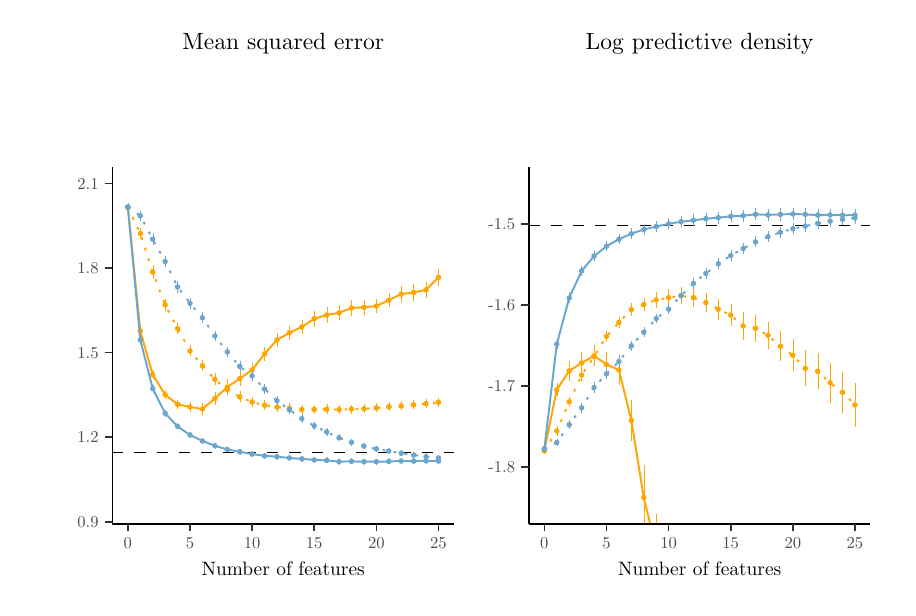
\begin{tikzpicture}[x=1pt,y=1pt]
\definecolor{fillColor}{RGB}{255,255,255}
\path[use as bounding box,fill=fillColor,fill opacity=0.00] (0,0) rectangle (310.76,202.36);
\begin{scope}
\path[clip] (  0.00,154.49) rectangle (160.26,202.36);
\definecolor{drawColor}{RGB}{255,255,255}
\definecolor{fillColor}{RGB}{255,255,255}

\path[draw=drawColor,line width= 0.6pt,line join=round,line cap=round,fill=fillColor] ( -0.00,154.49) rectangle (160.26,202.36);
\end{scope}
\begin{scope}
\path[clip] (  0.00,  0.00) rectangle (160.26,154.49);
\definecolor{drawColor}{RGB}{255,255,255}
\definecolor{fillColor}{RGB}{255,255,255}

\path[draw=drawColor,line width= 0.6pt,line join=round,line cap=round,fill=fillColor] ( -0.00,  0.00) rectangle (160.26,154.49);
\end{scope}
\begin{scope}
\path[clip] (160.26,154.49) rectangle (310.76,202.36);
\definecolor{drawColor}{RGB}{255,255,255}
\definecolor{fillColor}{RGB}{255,255,255}

\path[draw=drawColor,line width= 0.6pt,line join=round,line cap=round,fill=fillColor] (160.26,154.49) rectangle (310.76,202.36);
\end{scope}
\begin{scope}
\path[clip] (160.26,  0.00) rectangle (310.76,154.49);
\definecolor{drawColor}{RGB}{255,255,255}
\definecolor{fillColor}{RGB}{255,255,255}

\path[draw=drawColor,line width= 0.6pt,line join=round,line cap=round,fill=fillColor] (160.26,  0.00) rectangle (310.76,154.49);
\end{scope}
\begin{scope}
\path[clip] ( 30.60,157.24) rectangle (154.05,202.36);
\definecolor{drawColor}{RGB}{0,0,0}

\node[text=drawColor,anchor=base,inner sep=0pt, outer sep=0pt, scale=  0.85] at ( 92.32,194.43) {Mean squared error};
\end{scope}
\begin{scope}
\path[clip] ( 30.60, 23.07) rectangle (154.05,151.96);
\definecolor{fillColor}{RGB}{255,255,255}

\path[fill=fillColor] ( 30.60, 23.07) rectangle (154.05,151.96);
\definecolor{drawColor}{RGB}{0,0,0}

\path[draw=drawColor,line width= 0.3pt,dash pattern=on 4pt off 4pt ,line join=round] ( 30.60, 48.91) -- (154.05, 48.91);
\definecolor{drawColor}{RGB}{255,165,0}

\path[draw=drawColor,line width= 0.7pt,dash pattern=on 1pt off 3pt ,line join=round] ( 36.21,137.56) --
	( 40.70,127.95) --
	( 45.18,114.00) --
	( 49.67,102.23) --
	( 54.16, 93.63) --
	( 58.65, 85.55) --
	( 63.14, 80.20) --
	( 67.63, 75.31) --
	( 72.12, 71.57) --
	( 76.61, 68.94) --
	( 81.10, 67.10) --
	( 85.59, 65.94) --
	( 90.08, 65.27) --
	( 94.57, 64.82) --
	( 99.06, 64.37) --
	(103.54, 64.39) --
	(108.03, 64.47) --
	(112.52, 64.35) --
	(117.01, 64.52) --
	(121.50, 64.64) --
	(125.99, 64.94) --
	(130.48, 65.35) --
	(134.97, 65.67) --
	(139.46, 66.07) --
	(143.95, 66.51) --
	(148.44, 66.99);
\definecolor{fillColor}{RGB}{255,165,0}

\path[draw=drawColor,line width= 0.4pt,line join=round,line cap=round,fill=fillColor] ( 36.21,137.56) circle (  0.78);

\path[draw=drawColor,line width= 0.4pt,line join=round,line cap=round,fill=fillColor] ( 40.70,127.95) circle (  0.78);

\path[draw=drawColor,line width= 0.4pt,line join=round,line cap=round,fill=fillColor] ( 45.18,114.00) circle (  0.78);

\path[draw=drawColor,line width= 0.4pt,line join=round,line cap=round,fill=fillColor] ( 49.67,102.23) circle (  0.78);

\path[draw=drawColor,line width= 0.4pt,line join=round,line cap=round,fill=fillColor] ( 54.16, 93.63) circle (  0.78);

\path[draw=drawColor,line width= 0.4pt,line join=round,line cap=round,fill=fillColor] ( 58.65, 85.55) circle (  0.78);

\path[draw=drawColor,line width= 0.4pt,line join=round,line cap=round,fill=fillColor] ( 63.14, 80.20) circle (  0.78);

\path[draw=drawColor,line width= 0.4pt,line join=round,line cap=round,fill=fillColor] ( 67.63, 75.31) circle (  0.78);

\path[draw=drawColor,line width= 0.4pt,line join=round,line cap=round,fill=fillColor] ( 72.12, 71.57) circle (  0.78);

\path[draw=drawColor,line width= 0.4pt,line join=round,line cap=round,fill=fillColor] ( 76.61, 68.94) circle (  0.78);

\path[draw=drawColor,line width= 0.4pt,line join=round,line cap=round,fill=fillColor] ( 81.10, 67.10) circle (  0.78);

\path[draw=drawColor,line width= 0.4pt,line join=round,line cap=round,fill=fillColor] ( 85.59, 65.94) circle (  0.78);

\path[draw=drawColor,line width= 0.4pt,line join=round,line cap=round,fill=fillColor] ( 90.08, 65.27) circle (  0.78);

\path[draw=drawColor,line width= 0.4pt,line join=round,line cap=round,fill=fillColor] ( 94.57, 64.82) circle (  0.78);

\path[draw=drawColor,line width= 0.4pt,line join=round,line cap=round,fill=fillColor] ( 99.06, 64.37) circle (  0.78);

\path[draw=drawColor,line width= 0.4pt,line join=round,line cap=round,fill=fillColor] (103.54, 64.39) circle (  0.78);

\path[draw=drawColor,line width= 0.4pt,line join=round,line cap=round,fill=fillColor] (108.03, 64.47) circle (  0.78);

\path[draw=drawColor,line width= 0.4pt,line join=round,line cap=round,fill=fillColor] (112.52, 64.35) circle (  0.78);

\path[draw=drawColor,line width= 0.4pt,line join=round,line cap=round,fill=fillColor] (117.01, 64.52) circle (  0.78);

\path[draw=drawColor,line width= 0.4pt,line join=round,line cap=round,fill=fillColor] (121.50, 64.64) circle (  0.78);

\path[draw=drawColor,line width= 0.4pt,line join=round,line cap=round,fill=fillColor] (125.99, 64.94) circle (  0.78);

\path[draw=drawColor,line width= 0.4pt,line join=round,line cap=round,fill=fillColor] (130.48, 65.35) circle (  0.78);

\path[draw=drawColor,line width= 0.4pt,line join=round,line cap=round,fill=fillColor] (134.97, 65.67) circle (  0.78);

\path[draw=drawColor,line width= 0.4pt,line join=round,line cap=round,fill=fillColor] (139.46, 66.07) circle (  0.78);

\path[draw=drawColor,line width= 0.4pt,line join=round,line cap=round,fill=fillColor] (143.95, 66.51) circle (  0.78);

\path[draw=drawColor,line width= 0.4pt,line join=round,line cap=round,fill=fillColor] (148.44, 66.99) circle (  0.78);

\path[draw=drawColor,line width= 0.1pt,line join=round] ( 36.21,139.07) --
	( 36.21,139.07);

\path[draw=drawColor,line width= 0.1pt,line join=round] ( 36.21,139.07) --
	( 36.21,136.06);

\path[draw=drawColor,line width= 0.1pt,line join=round] ( 36.21,136.06) --
	( 36.21,136.06);

\path[draw=drawColor,line width= 0.1pt,line join=round] ( 40.70,130.02) --
	( 40.70,130.02);

\path[draw=drawColor,line width= 0.1pt,line join=round] ( 40.70,130.02) --
	( 40.70,125.87);

\path[draw=drawColor,line width= 0.1pt,line join=round] ( 40.70,125.87) --
	( 40.70,125.87);

\path[draw=drawColor,line width= 0.1pt,line join=round] ( 45.18,116.42) --
	( 45.18,116.42);

\path[draw=drawColor,line width= 0.1pt,line join=round] ( 45.18,116.42) --
	( 45.18,111.59);

\path[draw=drawColor,line width= 0.1pt,line join=round] ( 45.18,111.59) --
	( 45.18,111.59);

\path[draw=drawColor,line width= 0.1pt,line join=round] ( 49.67,104.48) --
	( 49.67,104.48);

\path[draw=drawColor,line width= 0.1pt,line join=round] ( 49.67,104.48) --
	( 49.67, 99.98);

\path[draw=drawColor,line width= 0.1pt,line join=round] ( 49.67, 99.98) --
	( 49.67, 99.98);

\path[draw=drawColor,line width= 0.1pt,line join=round] ( 54.16, 95.67) --
	( 54.16, 95.67);

\path[draw=drawColor,line width= 0.1pt,line join=round] ( 54.16, 95.67) --
	( 54.16, 91.60);

\path[draw=drawColor,line width= 0.1pt,line join=round] ( 54.16, 91.60) --
	( 54.16, 91.60);

\path[draw=drawColor,line width= 0.1pt,line join=round] ( 58.65, 87.54) --
	( 58.65, 87.54);

\path[draw=drawColor,line width= 0.1pt,line join=round] ( 58.65, 87.54) --
	( 58.65, 83.55);

\path[draw=drawColor,line width= 0.1pt,line join=round] ( 58.65, 83.55) --
	( 58.65, 83.55);

\path[draw=drawColor,line width= 0.1pt,line join=round] ( 63.14, 82.21) --
	( 63.14, 82.21);

\path[draw=drawColor,line width= 0.1pt,line join=round] ( 63.14, 82.21) --
	( 63.14, 78.20);

\path[draw=drawColor,line width= 0.1pt,line join=round] ( 63.14, 78.20) --
	( 63.14, 78.20);

\path[draw=drawColor,line width= 0.1pt,line join=round] ( 67.63, 77.42) --
	( 67.63, 77.42);

\path[draw=drawColor,line width= 0.1pt,line join=round] ( 67.63, 77.42) --
	( 67.63, 73.19);

\path[draw=drawColor,line width= 0.1pt,line join=round] ( 67.63, 73.19) --
	( 67.63, 73.19);

\path[draw=drawColor,line width= 0.1pt,line join=round] ( 72.12, 73.63) --
	( 72.12, 73.63);

\path[draw=drawColor,line width= 0.1pt,line join=round] ( 72.12, 73.63) --
	( 72.12, 69.51);

\path[draw=drawColor,line width= 0.1pt,line join=round] ( 72.12, 69.51) --
	( 72.12, 69.51);

\path[draw=drawColor,line width= 0.1pt,line join=round] ( 76.61, 70.92) --
	( 76.61, 70.92);

\path[draw=drawColor,line width= 0.1pt,line join=round] ( 76.61, 70.92) --
	( 76.61, 66.96);

\path[draw=drawColor,line width= 0.1pt,line join=round] ( 76.61, 66.96) --
	( 76.61, 66.96);

\path[draw=drawColor,line width= 0.1pt,line join=round] ( 81.10, 68.97) --
	( 81.10, 68.97);

\path[draw=drawColor,line width= 0.1pt,line join=round] ( 81.10, 68.97) --
	( 81.10, 65.24);

\path[draw=drawColor,line width= 0.1pt,line join=round] ( 81.10, 65.24) --
	( 81.10, 65.24);

\path[draw=drawColor,line width= 0.1pt,line join=round] ( 85.59, 67.82) --
	( 85.59, 67.82);

\path[draw=drawColor,line width= 0.1pt,line join=round] ( 85.59, 67.82) --
	( 85.59, 64.06);

\path[draw=drawColor,line width= 0.1pt,line join=round] ( 85.59, 64.06) --
	( 85.59, 64.06);

\path[draw=drawColor,line width= 0.1pt,line join=round] ( 90.08, 67.07) --
	( 90.08, 67.07);

\path[draw=drawColor,line width= 0.1pt,line join=round] ( 90.08, 67.07) --
	( 90.08, 63.46);

\path[draw=drawColor,line width= 0.1pt,line join=round] ( 90.08, 63.46) --
	( 90.08, 63.46);

\path[draw=drawColor,line width= 0.1pt,line join=round] ( 94.57, 66.60) --
	( 94.57, 66.60);

\path[draw=drawColor,line width= 0.1pt,line join=round] ( 94.57, 66.60) --
	( 94.57, 63.04);

\path[draw=drawColor,line width= 0.1pt,line join=round] ( 94.57, 63.04) --
	( 94.57, 63.04);

\path[draw=drawColor,line width= 0.1pt,line join=round] ( 99.06, 66.13) --
	( 99.06, 66.13);

\path[draw=drawColor,line width= 0.1pt,line join=round] ( 99.06, 66.13) --
	( 99.06, 62.60);

\path[draw=drawColor,line width= 0.1pt,line join=round] ( 99.06, 62.60) --
	( 99.06, 62.60);

\path[draw=drawColor,line width= 0.1pt,line join=round] (103.54, 66.13) --
	(103.54, 66.13);

\path[draw=drawColor,line width= 0.1pt,line join=round] (103.54, 66.13) --
	(103.54, 62.65);

\path[draw=drawColor,line width= 0.1pt,line join=round] (103.54, 62.65) --
	(103.54, 62.65);

\path[draw=drawColor,line width= 0.1pt,line join=round] (108.03, 66.21) --
	(108.03, 66.21);

\path[draw=drawColor,line width= 0.1pt,line join=round] (108.03, 66.21) --
	(108.03, 62.73);

\path[draw=drawColor,line width= 0.1pt,line join=round] (108.03, 62.73) --
	(108.03, 62.73);

\path[draw=drawColor,line width= 0.1pt,line join=round] (112.52, 66.03) --
	(112.52, 66.03);

\path[draw=drawColor,line width= 0.1pt,line join=round] (112.52, 66.03) --
	(112.52, 62.66);

\path[draw=drawColor,line width= 0.1pt,line join=round] (112.52, 62.66) --
	(112.52, 62.66);

\path[draw=drawColor,line width= 0.1pt,line join=round] (117.01, 66.19) --
	(117.01, 66.19);

\path[draw=drawColor,line width= 0.1pt,line join=round] (117.01, 66.19) --
	(117.01, 62.84);

\path[draw=drawColor,line width= 0.1pt,line join=round] (117.01, 62.84) --
	(117.01, 62.84);

\path[draw=drawColor,line width= 0.1pt,line join=round] (121.50, 66.27) --
	(121.50, 66.27);

\path[draw=drawColor,line width= 0.1pt,line join=round] (121.50, 66.27) --
	(121.50, 63.00);

\path[draw=drawColor,line width= 0.1pt,line join=round] (121.50, 63.00) --
	(121.50, 63.00);

\path[draw=drawColor,line width= 0.1pt,line join=round] (125.99, 66.58) --
	(125.99, 66.58);

\path[draw=drawColor,line width= 0.1pt,line join=round] (125.99, 66.58) --
	(125.99, 63.31);

\path[draw=drawColor,line width= 0.1pt,line join=round] (125.99, 63.31) --
	(125.99, 63.31);

\path[draw=drawColor,line width= 0.1pt,line join=round] (130.48, 67.00) --
	(130.48, 67.00);

\path[draw=drawColor,line width= 0.1pt,line join=round] (130.48, 67.00) --
	(130.48, 63.70);

\path[draw=drawColor,line width= 0.1pt,line join=round] (130.48, 63.70) --
	(130.48, 63.70);

\path[draw=drawColor,line width= 0.1pt,line join=round] (134.97, 67.31) --
	(134.97, 67.31);

\path[draw=drawColor,line width= 0.1pt,line join=round] (134.97, 67.31) --
	(134.97, 64.03);

\path[draw=drawColor,line width= 0.1pt,line join=round] (134.97, 64.03) --
	(134.97, 64.03);

\path[draw=drawColor,line width= 0.1pt,line join=round] (139.46, 67.70) --
	(139.46, 67.70);

\path[draw=drawColor,line width= 0.1pt,line join=round] (139.46, 67.70) --
	(139.46, 64.44);

\path[draw=drawColor,line width= 0.1pt,line join=round] (139.46, 64.44) --
	(139.46, 64.44);

\path[draw=drawColor,line width= 0.1pt,line join=round] (143.95, 68.15) --
	(143.95, 68.15);

\path[draw=drawColor,line width= 0.1pt,line join=round] (143.95, 68.15) --
	(143.95, 64.87);

\path[draw=drawColor,line width= 0.1pt,line join=round] (143.95, 64.87) --
	(143.95, 64.87);

\path[draw=drawColor,line width= 0.1pt,line join=round] (148.44, 68.64) --
	(148.44, 68.64);

\path[draw=drawColor,line width= 0.1pt,line join=round] (148.44, 68.64) --
	(148.44, 65.34);

\path[draw=drawColor,line width= 0.1pt,line join=round] (148.44, 65.34) --
	(148.44, 65.34);

\path[draw=drawColor,line width= 0.7pt,line join=round] ( 36.21,137.47) --
	( 40.70, 92.81) --
	( 45.18, 76.98) --
	( 49.67, 69.72) --
	( 54.16, 66.27) --
	( 58.65, 65.28) --
	( 63.14, 64.59) --
	( 67.63, 68.33) --
	( 72.12, 72.48) --
	( 76.61, 75.53) --
	( 81.10, 78.68) --
	( 85.59, 84.47) --
	( 90.08, 89.50) --
	( 94.57, 92.10) --
	( 99.06, 94.22) --
	(103.54, 97.18) --
	(108.03, 98.55) --
	(112.52, 99.30) --
	(117.01,101.07) --
	(121.50,101.31) --
	(125.99,101.78) --
	(130.48,103.87) --
	(134.97,106.09) --
	(139.46,106.67) --
	(143.95,107.64) --
	(148.44,112.14);

\path[draw=drawColor,line width= 0.4pt,line join=round,line cap=round,fill=fillColor] ( 36.21,137.47) circle (  0.78);

\path[draw=drawColor,line width= 0.4pt,line join=round,line cap=round,fill=fillColor] ( 40.70, 92.81) circle (  0.78);

\path[draw=drawColor,line width= 0.4pt,line join=round,line cap=round,fill=fillColor] ( 45.18, 76.98) circle (  0.78);

\path[draw=drawColor,line width= 0.4pt,line join=round,line cap=round,fill=fillColor] ( 49.67, 69.72) circle (  0.78);

\path[draw=drawColor,line width= 0.4pt,line join=round,line cap=round,fill=fillColor] ( 54.16, 66.27) circle (  0.78);

\path[draw=drawColor,line width= 0.4pt,line join=round,line cap=round,fill=fillColor] ( 58.65, 65.28) circle (  0.78);

\path[draw=drawColor,line width= 0.4pt,line join=round,line cap=round,fill=fillColor] ( 63.14, 64.59) circle (  0.78);

\path[draw=drawColor,line width= 0.4pt,line join=round,line cap=round,fill=fillColor] ( 67.63, 68.33) circle (  0.78);

\path[draw=drawColor,line width= 0.4pt,line join=round,line cap=round,fill=fillColor] ( 72.12, 72.48) circle (  0.78);

\path[draw=drawColor,line width= 0.4pt,line join=round,line cap=round,fill=fillColor] ( 76.61, 75.53) circle (  0.78);

\path[draw=drawColor,line width= 0.4pt,line join=round,line cap=round,fill=fillColor] ( 81.10, 78.68) circle (  0.78);

\path[draw=drawColor,line width= 0.4pt,line join=round,line cap=round,fill=fillColor] ( 85.59, 84.47) circle (  0.78);

\path[draw=drawColor,line width= 0.4pt,line join=round,line cap=round,fill=fillColor] ( 90.08, 89.50) circle (  0.78);

\path[draw=drawColor,line width= 0.4pt,line join=round,line cap=round,fill=fillColor] ( 94.57, 92.10) circle (  0.78);

\path[draw=drawColor,line width= 0.4pt,line join=round,line cap=round,fill=fillColor] ( 99.06, 94.22) circle (  0.78);

\path[draw=drawColor,line width= 0.4pt,line join=round,line cap=round,fill=fillColor] (103.54, 97.18) circle (  0.78);

\path[draw=drawColor,line width= 0.4pt,line join=round,line cap=round,fill=fillColor] (108.03, 98.55) circle (  0.78);

\path[draw=drawColor,line width= 0.4pt,line join=round,line cap=round,fill=fillColor] (112.52, 99.30) circle (  0.78);

\path[draw=drawColor,line width= 0.4pt,line join=round,line cap=round,fill=fillColor] (117.01,101.07) circle (  0.78);

\path[draw=drawColor,line width= 0.4pt,line join=round,line cap=round,fill=fillColor] (121.50,101.31) circle (  0.78);

\path[draw=drawColor,line width= 0.4pt,line join=round,line cap=round,fill=fillColor] (125.99,101.78) circle (  0.78);

\path[draw=drawColor,line width= 0.4pt,line join=round,line cap=round,fill=fillColor] (130.48,103.87) circle (  0.78);

\path[draw=drawColor,line width= 0.4pt,line join=round,line cap=round,fill=fillColor] (134.97,106.09) circle (  0.78);

\path[draw=drawColor,line width= 0.4pt,line join=round,line cap=round,fill=fillColor] (139.46,106.67) circle (  0.78);

\path[draw=drawColor,line width= 0.4pt,line join=round,line cap=round,fill=fillColor] (143.95,107.64) circle (  0.78);

\path[draw=drawColor,line width= 0.4pt,line join=round,line cap=round,fill=fillColor] (148.44,112.14) circle (  0.78);

\path[draw=drawColor,line width= 0.1pt,line join=round] ( 36.21,138.97) --
	( 36.21,138.97);

\path[draw=drawColor,line width= 0.1pt,line join=round] ( 36.21,138.97) --
	( 36.21,135.98);

\path[draw=drawColor,line width= 0.1pt,line join=round] ( 36.21,135.98) --
	( 36.21,135.98);

\path[draw=drawColor,line width= 0.1pt,line join=round] ( 40.70, 94.33) --
	( 40.70, 94.33);

\path[draw=drawColor,line width= 0.1pt,line join=round] ( 40.70, 94.33) --
	( 40.70, 91.30);

\path[draw=drawColor,line width= 0.1pt,line join=round] ( 40.70, 91.30) --
	( 40.70, 91.30);

\path[draw=drawColor,line width= 0.1pt,line join=round] ( 45.18, 78.52) --
	( 45.18, 78.52);

\path[draw=drawColor,line width= 0.1pt,line join=round] ( 45.18, 78.52) --
	( 45.18, 75.44);

\path[draw=drawColor,line width= 0.1pt,line join=round] ( 45.18, 75.44) --
	( 45.18, 75.44);

\path[draw=drawColor,line width= 0.1pt,line join=round] ( 49.67, 71.27) --
	( 49.67, 71.27);

\path[draw=drawColor,line width= 0.1pt,line join=round] ( 49.67, 71.27) --
	( 49.67, 68.16);

\path[draw=drawColor,line width= 0.1pt,line join=round] ( 49.67, 68.16) --
	( 49.67, 68.16);

\path[draw=drawColor,line width= 0.1pt,line join=round] ( 54.16, 67.97) --
	( 54.16, 67.97);

\path[draw=drawColor,line width= 0.1pt,line join=round] ( 54.16, 67.97) --
	( 54.16, 64.58);

\path[draw=drawColor,line width= 0.1pt,line join=round] ( 54.16, 64.58) --
	( 54.16, 64.58);

\path[draw=drawColor,line width= 0.1pt,line join=round] ( 58.65, 67.17) --
	( 58.65, 67.17);

\path[draw=drawColor,line width= 0.1pt,line join=round] ( 58.65, 67.17) --
	( 58.65, 63.40);

\path[draw=drawColor,line width= 0.1pt,line join=round] ( 58.65, 63.40) --
	( 58.65, 63.40);

\path[draw=drawColor,line width= 0.1pt,line join=round] ( 63.14, 66.64) --
	( 63.14, 66.64);

\path[draw=drawColor,line width= 0.1pt,line join=round] ( 63.14, 66.64) --
	( 63.14, 62.54);

\path[draw=drawColor,line width= 0.1pt,line join=round] ( 63.14, 62.54) --
	( 63.14, 62.54);

\path[draw=drawColor,line width= 0.1pt,line join=round] ( 67.63, 70.80) --
	( 67.63, 70.80);

\path[draw=drawColor,line width= 0.1pt,line join=round] ( 67.63, 70.80) --
	( 67.63, 65.86);

\path[draw=drawColor,line width= 0.1pt,line join=round] ( 67.63, 65.86) --
	( 67.63, 65.86);

\path[draw=drawColor,line width= 0.1pt,line join=round] ( 72.12, 75.23) --
	( 72.12, 75.23);

\path[draw=drawColor,line width= 0.1pt,line join=round] ( 72.12, 75.23) --
	( 72.12, 69.73);

\path[draw=drawColor,line width= 0.1pt,line join=round] ( 72.12, 69.73) --
	( 72.12, 69.73);

\path[draw=drawColor,line width= 0.1pt,line join=round] ( 76.61, 78.12) --
	( 76.61, 78.12);

\path[draw=drawColor,line width= 0.1pt,line join=round] ( 76.61, 78.12) --
	( 76.61, 72.94);

\path[draw=drawColor,line width= 0.1pt,line join=round] ( 76.61, 72.94) --
	( 76.61, 72.94);

\path[draw=drawColor,line width= 0.1pt,line join=round] ( 81.10, 81.18) --
	( 81.10, 81.18);

\path[draw=drawColor,line width= 0.1pt,line join=round] ( 81.10, 81.18) --
	( 81.10, 76.18);

\path[draw=drawColor,line width= 0.1pt,line join=round] ( 81.10, 76.18) --
	( 81.10, 76.18);

\path[draw=drawColor,line width= 0.1pt,line join=round] ( 85.59, 87.04) --
	( 85.59, 87.04);

\path[draw=drawColor,line width= 0.1pt,line join=round] ( 85.59, 87.04) --
	( 85.59, 81.89);

\path[draw=drawColor,line width= 0.1pt,line join=round] ( 85.59, 81.89) --
	( 85.59, 81.89);

\path[draw=drawColor,line width= 0.1pt,line join=round] ( 90.08, 91.88) --
	( 90.08, 91.88);

\path[draw=drawColor,line width= 0.1pt,line join=round] ( 90.08, 91.88) --
	( 90.08, 87.11);

\path[draw=drawColor,line width= 0.1pt,line join=round] ( 90.08, 87.11) --
	( 90.08, 87.11);

\path[draw=drawColor,line width= 0.1pt,line join=round] ( 94.57, 94.57) --
	( 94.57, 94.57);

\path[draw=drawColor,line width= 0.1pt,line join=round] ( 94.57, 94.57) --
	( 94.57, 89.64);

\path[draw=drawColor,line width= 0.1pt,line join=round] ( 94.57, 89.64) --
	( 94.57, 89.64);

\path[draw=drawColor,line width= 0.1pt,line join=round] ( 99.06, 96.86) --
	( 99.06, 96.86);

\path[draw=drawColor,line width= 0.1pt,line join=round] ( 99.06, 96.86) --
	( 99.06, 91.58);

\path[draw=drawColor,line width= 0.1pt,line join=round] ( 99.06, 91.58) --
	( 99.06, 91.58);

\path[draw=drawColor,line width= 0.1pt,line join=round] (103.54,100.03) --
	(103.54,100.03);

\path[draw=drawColor,line width= 0.1pt,line join=round] (103.54,100.03) --
	(103.54, 94.33);

\path[draw=drawColor,line width= 0.1pt,line join=round] (103.54, 94.33) --
	(103.54, 94.33);

\path[draw=drawColor,line width= 0.1pt,line join=round] (108.03,101.28) --
	(108.03,101.28);

\path[draw=drawColor,line width= 0.1pt,line join=round] (108.03,101.28) --
	(108.03, 95.82);

\path[draw=drawColor,line width= 0.1pt,line join=round] (108.03, 95.82) --
	(108.03, 95.82);

\path[draw=drawColor,line width= 0.1pt,line join=round] (112.52,102.03) --
	(112.52,102.03);

\path[draw=drawColor,line width= 0.1pt,line join=round] (112.52,102.03) --
	(112.52, 96.57);

\path[draw=drawColor,line width= 0.1pt,line join=round] (112.52, 96.57) --
	(112.52, 96.57);

\path[draw=drawColor,line width= 0.1pt,line join=round] (117.01,103.93) --
	(117.01,103.93);

\path[draw=drawColor,line width= 0.1pt,line join=round] (117.01,103.93) --
	(117.01, 98.21);

\path[draw=drawColor,line width= 0.1pt,line join=round] (117.01, 98.21) --
	(117.01, 98.21);

\path[draw=drawColor,line width= 0.1pt,line join=round] (121.50,103.92) --
	(121.50,103.92);

\path[draw=drawColor,line width= 0.1pt,line join=round] (121.50,103.92) --
	(121.50, 98.71);

\path[draw=drawColor,line width= 0.1pt,line join=round] (121.50, 98.71) --
	(121.50, 98.71);

\path[draw=drawColor,line width= 0.1pt,line join=round] (125.99,104.29) --
	(125.99,104.29);

\path[draw=drawColor,line width= 0.1pt,line join=round] (125.99,104.29) --
	(125.99, 99.27);

\path[draw=drawColor,line width= 0.1pt,line join=round] (125.99, 99.27) --
	(125.99, 99.27);

\path[draw=drawColor,line width= 0.1pt,line join=round] (130.48,106.46) --
	(130.48,106.46);

\path[draw=drawColor,line width= 0.1pt,line join=round] (130.48,106.46) --
	(130.48,101.27);

\path[draw=drawColor,line width= 0.1pt,line join=round] (130.48,101.27) --
	(130.48,101.27);

\path[draw=drawColor,line width= 0.1pt,line join=round] (134.97,108.86) --
	(134.97,108.86);

\path[draw=drawColor,line width= 0.1pt,line join=round] (134.97,108.86) --
	(134.97,103.31);

\path[draw=drawColor,line width= 0.1pt,line join=round] (134.97,103.31) --
	(134.97,103.31);

\path[draw=drawColor,line width= 0.1pt,line join=round] (139.46,109.57) --
	(139.46,109.57);

\path[draw=drawColor,line width= 0.1pt,line join=round] (139.46,109.57) --
	(139.46,103.77);

\path[draw=drawColor,line width= 0.1pt,line join=round] (139.46,103.77) --
	(139.46,103.77);

\path[draw=drawColor,line width= 0.1pt,line join=round] (143.95,110.50) --
	(143.95,110.50);

\path[draw=drawColor,line width= 0.1pt,line join=round] (143.95,110.50) --
	(143.95,104.78);

\path[draw=drawColor,line width= 0.1pt,line join=round] (143.95,104.78) --
	(143.95,104.78);

\path[draw=drawColor,line width= 0.1pt,line join=round] (148.44,115.33) --
	(148.44,115.33);

\path[draw=drawColor,line width= 0.1pt,line join=round] (148.44,115.33) --
	(148.44,108.95);

\path[draw=drawColor,line width= 0.1pt,line join=round] (148.44,108.95) --
	(148.44,108.95);
\definecolor{drawColor}{RGB}{108,166,205}

\path[draw=drawColor,line width= 0.7pt,dash pattern=on 1pt off 3pt ,line join=round] ( 36.21,137.57) --
	( 40.70,134.40) --
	( 45.18,125.92) --
	( 49.67,117.88) --
	( 54.16,108.69) --
	( 58.65,102.76) --
	( 63.14, 97.55) --
	( 67.63, 90.94) --
	( 72.12, 85.21) --
	( 76.61, 79.96) --
	( 81.10, 76.54) --
	( 85.59, 71.80) --
	( 90.08, 67.57) --
	( 94.57, 64.26) --
	( 99.06, 61.10) --
	(103.54, 58.48) --
	(108.03, 56.27) --
	(112.52, 54.16) --
	(117.01, 52.52) --
	(121.50, 51.17) --
	(125.99, 50.14) --
	(130.48, 49.37) --
	(134.97, 48.56) --
	(139.46, 47.92) --
	(143.95, 47.34) --
	(148.44, 46.88);
\definecolor{fillColor}{RGB}{108,166,205}

\path[draw=drawColor,line width= 0.4pt,line join=round,line cap=round,fill=fillColor] ( 36.21,137.57) circle (  0.78);

\path[draw=drawColor,line width= 0.4pt,line join=round,line cap=round,fill=fillColor] ( 40.70,134.40) circle (  0.78);

\path[draw=drawColor,line width= 0.4pt,line join=round,line cap=round,fill=fillColor] ( 45.18,125.92) circle (  0.78);

\path[draw=drawColor,line width= 0.4pt,line join=round,line cap=round,fill=fillColor] ( 49.67,117.88) circle (  0.78);

\path[draw=drawColor,line width= 0.4pt,line join=round,line cap=round,fill=fillColor] ( 54.16,108.69) circle (  0.78);

\path[draw=drawColor,line width= 0.4pt,line join=round,line cap=round,fill=fillColor] ( 58.65,102.76) circle (  0.78);

\path[draw=drawColor,line width= 0.4pt,line join=round,line cap=round,fill=fillColor] ( 63.14, 97.55) circle (  0.78);

\path[draw=drawColor,line width= 0.4pt,line join=round,line cap=round,fill=fillColor] ( 67.63, 90.94) circle (  0.78);

\path[draw=drawColor,line width= 0.4pt,line join=round,line cap=round,fill=fillColor] ( 72.12, 85.21) circle (  0.78);

\path[draw=drawColor,line width= 0.4pt,line join=round,line cap=round,fill=fillColor] ( 76.61, 79.96) circle (  0.78);

\path[draw=drawColor,line width= 0.4pt,line join=round,line cap=round,fill=fillColor] ( 81.10, 76.54) circle (  0.78);

\path[draw=drawColor,line width= 0.4pt,line join=round,line cap=round,fill=fillColor] ( 85.59, 71.80) circle (  0.78);

\path[draw=drawColor,line width= 0.4pt,line join=round,line cap=round,fill=fillColor] ( 90.08, 67.57) circle (  0.78);

\path[draw=drawColor,line width= 0.4pt,line join=round,line cap=round,fill=fillColor] ( 94.57, 64.26) circle (  0.78);

\path[draw=drawColor,line width= 0.4pt,line join=round,line cap=round,fill=fillColor] ( 99.06, 61.10) circle (  0.78);

\path[draw=drawColor,line width= 0.4pt,line join=round,line cap=round,fill=fillColor] (103.54, 58.48) circle (  0.78);

\path[draw=drawColor,line width= 0.4pt,line join=round,line cap=round,fill=fillColor] (108.03, 56.27) circle (  0.78);

\path[draw=drawColor,line width= 0.4pt,line join=round,line cap=round,fill=fillColor] (112.52, 54.16) circle (  0.78);

\path[draw=drawColor,line width= 0.4pt,line join=round,line cap=round,fill=fillColor] (117.01, 52.52) circle (  0.78);

\path[draw=drawColor,line width= 0.4pt,line join=round,line cap=round,fill=fillColor] (121.50, 51.17) circle (  0.78);

\path[draw=drawColor,line width= 0.4pt,line join=round,line cap=round,fill=fillColor] (125.99, 50.14) circle (  0.78);

\path[draw=drawColor,line width= 0.4pt,line join=round,line cap=round,fill=fillColor] (130.48, 49.37) circle (  0.78);

\path[draw=drawColor,line width= 0.4pt,line join=round,line cap=round,fill=fillColor] (134.97, 48.56) circle (  0.78);

\path[draw=drawColor,line width= 0.4pt,line join=round,line cap=round,fill=fillColor] (139.46, 47.92) circle (  0.78);

\path[draw=drawColor,line width= 0.4pt,line join=round,line cap=round,fill=fillColor] (143.95, 47.34) circle (  0.78);

\path[draw=drawColor,line width= 0.4pt,line join=round,line cap=round,fill=fillColor] (148.44, 46.88) circle (  0.78);

\path[draw=drawColor,line width= 0.1pt,line join=round] ( 36.21,139.08) --
	( 36.21,139.08);

\path[draw=drawColor,line width= 0.1pt,line join=round] ( 36.21,139.08) --
	( 36.21,136.07);

\path[draw=drawColor,line width= 0.1pt,line join=round] ( 36.21,136.07) --
	( 36.21,136.07);

\path[draw=drawColor,line width= 0.1pt,line join=round] ( 40.70,136.18) --
	( 40.70,136.18);

\path[draw=drawColor,line width= 0.1pt,line join=round] ( 40.70,136.18) --
	( 40.70,132.63);

\path[draw=drawColor,line width= 0.1pt,line join=round] ( 40.70,132.63) --
	( 40.70,132.63);

\path[draw=drawColor,line width= 0.1pt,line join=round] ( 45.18,127.99) --
	( 45.18,127.99);

\path[draw=drawColor,line width= 0.1pt,line join=round] ( 45.18,127.99) --
	( 45.18,123.84);

\path[draw=drawColor,line width= 0.1pt,line join=round] ( 45.18,123.84) --
	( 45.18,123.84);

\path[draw=drawColor,line width= 0.1pt,line join=round] ( 49.67,119.94) --
	( 49.67,119.94);

\path[draw=drawColor,line width= 0.1pt,line join=round] ( 49.67,119.94) --
	( 49.67,115.82);

\path[draw=drawColor,line width= 0.1pt,line join=round] ( 49.67,115.82) --
	( 49.67,115.82);

\path[draw=drawColor,line width= 0.1pt,line join=round] ( 54.16,110.77) --
	( 54.16,110.77);

\path[draw=drawColor,line width= 0.1pt,line join=round] ( 54.16,110.77) --
	( 54.16,106.62);

\path[draw=drawColor,line width= 0.1pt,line join=round] ( 54.16,106.62) --
	( 54.16,106.62);

\path[draw=drawColor,line width= 0.1pt,line join=round] ( 58.65,104.76) --
	( 58.65,104.76);

\path[draw=drawColor,line width= 0.1pt,line join=round] ( 58.65,104.76) --
	( 58.65,100.75);

\path[draw=drawColor,line width= 0.1pt,line join=round] ( 58.65,100.75) --
	( 58.65,100.75);

\path[draw=drawColor,line width= 0.1pt,line join=round] ( 63.14, 99.58) --
	( 63.14, 99.58);

\path[draw=drawColor,line width= 0.1pt,line join=round] ( 63.14, 99.58) --
	( 63.14, 95.52);

\path[draw=drawColor,line width= 0.1pt,line join=round] ( 63.14, 95.52) --
	( 63.14, 95.52);

\path[draw=drawColor,line width= 0.1pt,line join=round] ( 67.63, 92.80) --
	( 67.63, 92.80);

\path[draw=drawColor,line width= 0.1pt,line join=round] ( 67.63, 92.80) --
	( 67.63, 89.08);

\path[draw=drawColor,line width= 0.1pt,line join=round] ( 67.63, 89.08) --
	( 67.63, 89.08);

\path[draw=drawColor,line width= 0.1pt,line join=round] ( 72.12, 87.05) --
	( 72.12, 87.05);

\path[draw=drawColor,line width= 0.1pt,line join=round] ( 72.12, 87.05) --
	( 72.12, 83.36);

\path[draw=drawColor,line width= 0.1pt,line join=round] ( 72.12, 83.36) --
	( 72.12, 83.36);

\path[draw=drawColor,line width= 0.1pt,line join=round] ( 76.61, 81.74) --
	( 76.61, 81.74);

\path[draw=drawColor,line width= 0.1pt,line join=round] ( 76.61, 81.74) --
	( 76.61, 78.17);

\path[draw=drawColor,line width= 0.1pt,line join=round] ( 76.61, 78.17) --
	( 76.61, 78.17);

\path[draw=drawColor,line width= 0.1pt,line join=round] ( 81.10, 78.24) --
	( 81.10, 78.24);

\path[draw=drawColor,line width= 0.1pt,line join=round] ( 81.10, 78.24) --
	( 81.10, 74.84);

\path[draw=drawColor,line width= 0.1pt,line join=round] ( 81.10, 74.84) --
	( 81.10, 74.84);

\path[draw=drawColor,line width= 0.1pt,line join=round] ( 85.59, 73.48) --
	( 85.59, 73.48);

\path[draw=drawColor,line width= 0.1pt,line join=round] ( 85.59, 73.48) --
	( 85.59, 70.13);

\path[draw=drawColor,line width= 0.1pt,line join=round] ( 85.59, 70.13) --
	( 85.59, 70.13);

\path[draw=drawColor,line width= 0.1pt,line join=round] ( 90.08, 69.19) --
	( 90.08, 69.19);

\path[draw=drawColor,line width= 0.1pt,line join=round] ( 90.08, 69.19) --
	( 90.08, 65.96);

\path[draw=drawColor,line width= 0.1pt,line join=round] ( 90.08, 65.96) --
	( 90.08, 65.96);

\path[draw=drawColor,line width= 0.1pt,line join=round] ( 94.57, 65.88) --
	( 94.57, 65.88);

\path[draw=drawColor,line width= 0.1pt,line join=round] ( 94.57, 65.88) --
	( 94.57, 62.65);

\path[draw=drawColor,line width= 0.1pt,line join=round] ( 94.57, 62.65) --
	( 94.57, 62.65);

\path[draw=drawColor,line width= 0.1pt,line join=round] ( 99.06, 62.60) --
	( 99.06, 62.60);

\path[draw=drawColor,line width= 0.1pt,line join=round] ( 99.06, 62.60) --
	( 99.06, 59.61);

\path[draw=drawColor,line width= 0.1pt,line join=round] ( 99.06, 59.61) --
	( 99.06, 59.61);

\path[draw=drawColor,line width= 0.1pt,line join=round] (103.54, 59.86) --
	(103.54, 59.86);

\path[draw=drawColor,line width= 0.1pt,line join=round] (103.54, 59.86) --
	(103.54, 57.10);

\path[draw=drawColor,line width= 0.1pt,line join=round] (103.54, 57.10) --
	(103.54, 57.10);

\path[draw=drawColor,line width= 0.1pt,line join=round] (108.03, 57.56) --
	(108.03, 57.56);

\path[draw=drawColor,line width= 0.1pt,line join=round] (108.03, 57.56) --
	(108.03, 54.98);

\path[draw=drawColor,line width= 0.1pt,line join=round] (108.03, 54.98) --
	(108.03, 54.98);

\path[draw=drawColor,line width= 0.1pt,line join=round] (112.52, 55.40) --
	(112.52, 55.40);

\path[draw=drawColor,line width= 0.1pt,line join=round] (112.52, 55.40) --
	(112.52, 52.93);

\path[draw=drawColor,line width= 0.1pt,line join=round] (112.52, 52.93) --
	(112.52, 52.93);

\path[draw=drawColor,line width= 0.1pt,line join=round] (117.01, 53.69) --
	(117.01, 53.69);

\path[draw=drawColor,line width= 0.1pt,line join=round] (117.01, 53.69) --
	(117.01, 51.36);

\path[draw=drawColor,line width= 0.1pt,line join=round] (117.01, 51.36) --
	(117.01, 51.36);

\path[draw=drawColor,line width= 0.1pt,line join=round] (121.50, 52.32) --
	(121.50, 52.32);

\path[draw=drawColor,line width= 0.1pt,line join=round] (121.50, 52.32) --
	(121.50, 50.01);

\path[draw=drawColor,line width= 0.1pt,line join=round] (121.50, 50.01) --
	(121.50, 50.01);

\path[draw=drawColor,line width= 0.1pt,line join=round] (125.99, 51.31) --
	(125.99, 51.31);

\path[draw=drawColor,line width= 0.1pt,line join=round] (125.99, 51.31) --
	(125.99, 48.97);

\path[draw=drawColor,line width= 0.1pt,line join=round] (125.99, 48.97) --
	(125.99, 48.97);

\path[draw=drawColor,line width= 0.1pt,line join=round] (130.48, 50.54) --
	(130.48, 50.54);

\path[draw=drawColor,line width= 0.1pt,line join=round] (130.48, 50.54) --
	(130.48, 48.20);

\path[draw=drawColor,line width= 0.1pt,line join=round] (130.48, 48.20) --
	(130.48, 48.20);

\path[draw=drawColor,line width= 0.1pt,line join=round] (134.97, 49.69) --
	(134.97, 49.69);

\path[draw=drawColor,line width= 0.1pt,line join=round] (134.97, 49.69) --
	(134.97, 47.42);

\path[draw=drawColor,line width= 0.1pt,line join=round] (134.97, 47.42) --
	(134.97, 47.42);

\path[draw=drawColor,line width= 0.1pt,line join=round] (139.46, 49.06) --
	(139.46, 49.06);

\path[draw=drawColor,line width= 0.1pt,line join=round] (139.46, 49.06) --
	(139.46, 46.78);

\path[draw=drawColor,line width= 0.1pt,line join=round] (139.46, 46.78) --
	(139.46, 46.78);

\path[draw=drawColor,line width= 0.1pt,line join=round] (143.95, 48.49) --
	(143.95, 48.49);

\path[draw=drawColor,line width= 0.1pt,line join=round] (143.95, 48.49) --
	(143.95, 46.19);

\path[draw=drawColor,line width= 0.1pt,line join=round] (143.95, 46.19) --
	(143.95, 46.19);

\path[draw=drawColor,line width= 0.1pt,line join=round] (148.44, 48.03) --
	(148.44, 48.03);

\path[draw=drawColor,line width= 0.1pt,line join=round] (148.44, 48.03) --
	(148.44, 45.73);

\path[draw=drawColor,line width= 0.1pt,line join=round] (148.44, 45.73) --
	(148.44, 45.73);

\path[draw=drawColor,line width= 0.7pt,line join=round] ( 36.21,137.48) --
	( 40.70, 89.56) --
	( 45.18, 71.94) --
	( 49.67, 63.01) --
	( 54.16, 58.27) --
	( 58.65, 55.20) --
	( 63.14, 53.02) --
	( 67.63, 51.29) --
	( 72.12, 49.96) --
	( 76.61, 49.13) --
	( 81.10, 48.27) --
	( 85.59, 47.64) --
	( 90.08, 47.33) --
	( 94.57, 46.87) --
	( 99.06, 46.54) --
	(103.54, 46.17) --
	(108.03, 46.00) --
	(112.52, 45.55) --
	(117.01, 45.63) --
	(121.50, 45.54) --
	(125.99, 45.52) --
	(130.48, 45.60) --
	(134.97, 45.79) --
	(139.46, 45.73) --
	(143.95, 45.83) --
	(148.44, 45.75);

\path[draw=drawColor,line width= 0.4pt,line join=round,line cap=round,fill=fillColor] ( 36.21,137.48) circle (  0.78);

\path[draw=drawColor,line width= 0.4pt,line join=round,line cap=round,fill=fillColor] ( 40.70, 89.56) circle (  0.78);

\path[draw=drawColor,line width= 0.4pt,line join=round,line cap=round,fill=fillColor] ( 45.18, 71.94) circle (  0.78);

\path[draw=drawColor,line width= 0.4pt,line join=round,line cap=round,fill=fillColor] ( 49.67, 63.01) circle (  0.78);

\path[draw=drawColor,line width= 0.4pt,line join=round,line cap=round,fill=fillColor] ( 54.16, 58.27) circle (  0.78);

\path[draw=drawColor,line width= 0.4pt,line join=round,line cap=round,fill=fillColor] ( 58.65, 55.20) circle (  0.78);

\path[draw=drawColor,line width= 0.4pt,line join=round,line cap=round,fill=fillColor] ( 63.14, 53.02) circle (  0.78);

\path[draw=drawColor,line width= 0.4pt,line join=round,line cap=round,fill=fillColor] ( 67.63, 51.29) circle (  0.78);

\path[draw=drawColor,line width= 0.4pt,line join=round,line cap=round,fill=fillColor] ( 72.12, 49.96) circle (  0.78);

\path[draw=drawColor,line width= 0.4pt,line join=round,line cap=round,fill=fillColor] ( 76.61, 49.13) circle (  0.78);

\path[draw=drawColor,line width= 0.4pt,line join=round,line cap=round,fill=fillColor] ( 81.10, 48.27) circle (  0.78);

\path[draw=drawColor,line width= 0.4pt,line join=round,line cap=round,fill=fillColor] ( 85.59, 47.64) circle (  0.78);

\path[draw=drawColor,line width= 0.4pt,line join=round,line cap=round,fill=fillColor] ( 90.08, 47.33) circle (  0.78);

\path[draw=drawColor,line width= 0.4pt,line join=round,line cap=round,fill=fillColor] ( 94.57, 46.87) circle (  0.78);

\path[draw=drawColor,line width= 0.4pt,line join=round,line cap=round,fill=fillColor] ( 99.06, 46.54) circle (  0.78);

\path[draw=drawColor,line width= 0.4pt,line join=round,line cap=round,fill=fillColor] (103.54, 46.17) circle (  0.78);

\path[draw=drawColor,line width= 0.4pt,line join=round,line cap=round,fill=fillColor] (108.03, 46.00) circle (  0.78);

\path[draw=drawColor,line width= 0.4pt,line join=round,line cap=round,fill=fillColor] (112.52, 45.55) circle (  0.78);

\path[draw=drawColor,line width= 0.4pt,line join=round,line cap=round,fill=fillColor] (117.01, 45.63) circle (  0.78);

\path[draw=drawColor,line width= 0.4pt,line join=round,line cap=round,fill=fillColor] (121.50, 45.54) circle (  0.78);

\path[draw=drawColor,line width= 0.4pt,line join=round,line cap=round,fill=fillColor] (125.99, 45.52) circle (  0.78);

\path[draw=drawColor,line width= 0.4pt,line join=round,line cap=round,fill=fillColor] (130.48, 45.60) circle (  0.78);

\path[draw=drawColor,line width= 0.4pt,line join=round,line cap=round,fill=fillColor] (134.97, 45.79) circle (  0.78);

\path[draw=drawColor,line width= 0.4pt,line join=round,line cap=round,fill=fillColor] (139.46, 45.73) circle (  0.78);

\path[draw=drawColor,line width= 0.4pt,line join=round,line cap=round,fill=fillColor] (143.95, 45.83) circle (  0.78);

\path[draw=drawColor,line width= 0.4pt,line join=round,line cap=round,fill=fillColor] (148.44, 45.75) circle (  0.78);

\path[draw=drawColor,line width= 0.1pt,line join=round] ( 36.21,138.97) --
	( 36.21,138.97);

\path[draw=drawColor,line width= 0.1pt,line join=round] ( 36.21,138.97) --
	( 36.21,135.99);

\path[draw=drawColor,line width= 0.1pt,line join=round] ( 36.21,135.99) --
	( 36.21,135.99);

\path[draw=drawColor,line width= 0.1pt,line join=round] ( 40.70, 91.26) --
	( 40.70, 91.26);

\path[draw=drawColor,line width= 0.1pt,line join=round] ( 40.70, 91.26) --
	( 40.70, 87.85);

\path[draw=drawColor,line width= 0.1pt,line join=round] ( 40.70, 87.85) --
	( 40.70, 87.85);

\path[draw=drawColor,line width= 0.1pt,line join=round] ( 45.18, 73.37) --
	( 45.18, 73.37);

\path[draw=drawColor,line width= 0.1pt,line join=round] ( 45.18, 73.37) --
	( 45.18, 70.52);

\path[draw=drawColor,line width= 0.1pt,line join=round] ( 45.18, 70.52) --
	( 45.18, 70.52);

\path[draw=drawColor,line width= 0.1pt,line join=round] ( 49.67, 64.17) --
	( 49.67, 64.17);

\path[draw=drawColor,line width= 0.1pt,line join=round] ( 49.67, 64.17) --
	( 49.67, 61.85);

\path[draw=drawColor,line width= 0.1pt,line join=round] ( 49.67, 61.85) --
	( 49.67, 61.85);

\path[draw=drawColor,line width= 0.1pt,line join=round] ( 54.16, 59.37) --
	( 54.16, 59.37);

\path[draw=drawColor,line width= 0.1pt,line join=round] ( 54.16, 59.37) --
	( 54.16, 57.17);

\path[draw=drawColor,line width= 0.1pt,line join=round] ( 54.16, 57.17) --
	( 54.16, 57.17);

\path[draw=drawColor,line width= 0.1pt,line join=round] ( 58.65, 56.28) --
	( 58.65, 56.28);

\path[draw=drawColor,line width= 0.1pt,line join=round] ( 58.65, 56.28) --
	( 58.65, 54.12);

\path[draw=drawColor,line width= 0.1pt,line join=round] ( 58.65, 54.12) --
	( 58.65, 54.12);

\path[draw=drawColor,line width= 0.1pt,line join=round] ( 63.14, 54.08) --
	( 63.14, 54.08);

\path[draw=drawColor,line width= 0.1pt,line join=round] ( 63.14, 54.08) --
	( 63.14, 51.97);

\path[draw=drawColor,line width= 0.1pt,line join=round] ( 63.14, 51.97) --
	( 63.14, 51.97);

\path[draw=drawColor,line width= 0.1pt,line join=round] ( 67.63, 52.36) --
	( 67.63, 52.36);

\path[draw=drawColor,line width= 0.1pt,line join=round] ( 67.63, 52.36) --
	( 67.63, 50.22);

\path[draw=drawColor,line width= 0.1pt,line join=round] ( 67.63, 50.22) --
	( 67.63, 50.22);

\path[draw=drawColor,line width= 0.1pt,line join=round] ( 72.12, 50.99) --
	( 72.12, 50.99);

\path[draw=drawColor,line width= 0.1pt,line join=round] ( 72.12, 50.99) --
	( 72.12, 48.93);

\path[draw=drawColor,line width= 0.1pt,line join=round] ( 72.12, 48.93) --
	( 72.12, 48.93);

\path[draw=drawColor,line width= 0.1pt,line join=round] ( 76.61, 50.17) --
	( 76.61, 50.17);

\path[draw=drawColor,line width= 0.1pt,line join=round] ( 76.61, 50.17) --
	( 76.61, 48.08);

\path[draw=drawColor,line width= 0.1pt,line join=round] ( 76.61, 48.08) --
	( 76.61, 48.08);

\path[draw=drawColor,line width= 0.1pt,line join=round] ( 81.10, 49.27) --
	( 81.10, 49.27);

\path[draw=drawColor,line width= 0.1pt,line join=round] ( 81.10, 49.27) --
	( 81.10, 47.27);

\path[draw=drawColor,line width= 0.1pt,line join=round] ( 81.10, 47.27) --
	( 81.10, 47.27);

\path[draw=drawColor,line width= 0.1pt,line join=round] ( 85.59, 48.64) --
	( 85.59, 48.64);

\path[draw=drawColor,line width= 0.1pt,line join=round] ( 85.59, 48.64) --
	( 85.59, 46.63);

\path[draw=drawColor,line width= 0.1pt,line join=round] ( 85.59, 46.63) --
	( 85.59, 46.63);

\path[draw=drawColor,line width= 0.1pt,line join=round] ( 90.08, 48.42) --
	( 90.08, 48.42);

\path[draw=drawColor,line width= 0.1pt,line join=round] ( 90.08, 48.42) --
	( 90.08, 46.25);

\path[draw=drawColor,line width= 0.1pt,line join=round] ( 90.08, 46.25) --
	( 90.08, 46.25);

\path[draw=drawColor,line width= 0.1pt,line join=round] ( 94.57, 47.94) --
	( 94.57, 47.94);

\path[draw=drawColor,line width= 0.1pt,line join=round] ( 94.57, 47.94) --
	( 94.57, 45.81);

\path[draw=drawColor,line width= 0.1pt,line join=round] ( 94.57, 45.81) --
	( 94.57, 45.81);

\path[draw=drawColor,line width= 0.1pt,line join=round] ( 99.06, 47.61) --
	( 99.06, 47.61);

\path[draw=drawColor,line width= 0.1pt,line join=round] ( 99.06, 47.61) --
	( 99.06, 45.47);

\path[draw=drawColor,line width= 0.1pt,line join=round] ( 99.06, 45.47) --
	( 99.06, 45.47);

\path[draw=drawColor,line width= 0.1pt,line join=round] (103.54, 47.26) --
	(103.54, 47.26);

\path[draw=drawColor,line width= 0.1pt,line join=round] (103.54, 47.26) --
	(103.54, 45.08);

\path[draw=drawColor,line width= 0.1pt,line join=round] (103.54, 45.08) --
	(103.54, 45.08);

\path[draw=drawColor,line width= 0.1pt,line join=round] (108.03, 47.08) --
	(108.03, 47.08);

\path[draw=drawColor,line width= 0.1pt,line join=round] (108.03, 47.08) --
	(108.03, 44.93);

\path[draw=drawColor,line width= 0.1pt,line join=round] (108.03, 44.93) --
	(108.03, 44.93);

\path[draw=drawColor,line width= 0.1pt,line join=round] (112.52, 46.63) --
	(112.52, 46.63);

\path[draw=drawColor,line width= 0.1pt,line join=round] (112.52, 46.63) --
	(112.52, 44.47);

\path[draw=drawColor,line width= 0.1pt,line join=round] (112.52, 44.47) --
	(112.52, 44.47);

\path[draw=drawColor,line width= 0.1pt,line join=round] (117.01, 46.68) --
	(117.01, 46.68);

\path[draw=drawColor,line width= 0.1pt,line join=round] (117.01, 46.68) --
	(117.01, 44.57);

\path[draw=drawColor,line width= 0.1pt,line join=round] (117.01, 44.57) --
	(117.01, 44.57);

\path[draw=drawColor,line width= 0.1pt,line join=round] (121.50, 46.62) --
	(121.50, 46.62);

\path[draw=drawColor,line width= 0.1pt,line join=round] (121.50, 46.62) --
	(121.50, 44.47);

\path[draw=drawColor,line width= 0.1pt,line join=round] (121.50, 44.47) --
	(121.50, 44.47);

\path[draw=drawColor,line width= 0.1pt,line join=round] (125.99, 46.60) --
	(125.99, 46.60);

\path[draw=drawColor,line width= 0.1pt,line join=round] (125.99, 46.60) --
	(125.99, 44.45);

\path[draw=drawColor,line width= 0.1pt,line join=round] (125.99, 44.45) --
	(125.99, 44.45);

\path[draw=drawColor,line width= 0.1pt,line join=round] (130.48, 46.68) --
	(130.48, 46.68);

\path[draw=drawColor,line width= 0.1pt,line join=round] (130.48, 46.68) --
	(130.48, 44.52);

\path[draw=drawColor,line width= 0.1pt,line join=round] (130.48, 44.52) --
	(130.48, 44.52);

\path[draw=drawColor,line width= 0.1pt,line join=round] (134.97, 46.90) --
	(134.97, 46.90);

\path[draw=drawColor,line width= 0.1pt,line join=round] (134.97, 46.90) --
	(134.97, 44.68);

\path[draw=drawColor,line width= 0.1pt,line join=round] (134.97, 44.68) --
	(134.97, 44.68);

\path[draw=drawColor,line width= 0.1pt,line join=round] (139.46, 46.83) --
	(139.46, 46.83);

\path[draw=drawColor,line width= 0.1pt,line join=round] (139.46, 46.83) --
	(139.46, 44.63);

\path[draw=drawColor,line width= 0.1pt,line join=round] (139.46, 44.63) --
	(139.46, 44.63);

\path[draw=drawColor,line width= 0.1pt,line join=round] (143.95, 46.95) --
	(143.95, 46.95);

\path[draw=drawColor,line width= 0.1pt,line join=round] (143.95, 46.95) --
	(143.95, 44.71);

\path[draw=drawColor,line width= 0.1pt,line join=round] (143.95, 44.71) --
	(143.95, 44.71);

\path[draw=drawColor,line width= 0.1pt,line join=round] (148.44, 46.86) --
	(148.44, 46.86);

\path[draw=drawColor,line width= 0.1pt,line join=round] (148.44, 46.86) --
	(148.44, 44.65);

\path[draw=drawColor,line width= 0.1pt,line join=round] (148.44, 44.65) --
	(148.44, 44.65);
\end{scope}
\begin{scope}
\path[clip] (181.09,157.24) rectangle (304.55,202.36);
\definecolor{drawColor}{RGB}{0,0,0}

\node[text=drawColor,anchor=base,inner sep=0pt, outer sep=0pt, scale=  0.85] at (242.82,194.43) {Log predictive density};
\end{scope}
\begin{scope}
\path[clip] (181.09, 23.07) rectangle (304.55,151.96);
\definecolor{fillColor}{RGB}{255,255,255}

\path[fill=fillColor] (181.09, 23.07) rectangle (304.55,151.96);
\definecolor{drawColor}{RGB}{0,0,0}

\path[draw=drawColor,line width= 0.3pt,dash pattern=on 4pt off 4pt ,line join=round] (181.09,130.79) -- (304.55,130.79);
\definecolor{drawColor}{RGB}{255,165,0}

\path[draw=drawColor,line width= 0.7pt,dash pattern=on 1pt off 3pt ,line join=round] (186.70, 49.48) --
	(191.19, 56.61) --
	(195.68, 67.14) --
	(200.17, 76.80) --
	(204.66, 83.51) --
	(209.15, 90.80) --
	(213.64, 95.87) --
	(218.13,100.49) --
	(222.62,102.32) --
	(227.11,103.99) --
	(231.60,104.80) --
	(236.09,105.47) --
	(240.57,104.82) --
	(245.06,103.05) --
	(249.55,100.62) --
	(254.04, 98.51) --
	(258.53, 94.59) --
	(263.02, 93.72) --
	(267.51, 91.19) --
	(272.00, 87.20) --
	(276.49, 84.01) --
	(280.98, 79.24) --
	(285.47, 78.16) --
	(289.96, 74.02) --
	(294.45, 70.61) --
	(298.93, 66.05);
\definecolor{fillColor}{RGB}{255,165,0}

\path[draw=drawColor,line width= 0.4pt,line join=round,line cap=round,fill=fillColor] (186.70, 49.48) circle (  0.78);

\path[draw=drawColor,line width= 0.4pt,line join=round,line cap=round,fill=fillColor] (191.19, 56.61) circle (  0.78);

\path[draw=drawColor,line width= 0.4pt,line join=round,line cap=round,fill=fillColor] (195.68, 67.14) circle (  0.78);

\path[draw=drawColor,line width= 0.4pt,line join=round,line cap=round,fill=fillColor] (200.17, 76.80) circle (  0.78);

\path[draw=drawColor,line width= 0.4pt,line join=round,line cap=round,fill=fillColor] (204.66, 83.51) circle (  0.78);

\path[draw=drawColor,line width= 0.4pt,line join=round,line cap=round,fill=fillColor] (209.15, 90.80) circle (  0.78);

\path[draw=drawColor,line width= 0.4pt,line join=round,line cap=round,fill=fillColor] (213.64, 95.87) circle (  0.78);

\path[draw=drawColor,line width= 0.4pt,line join=round,line cap=round,fill=fillColor] (218.13,100.49) circle (  0.78);

\path[draw=drawColor,line width= 0.4pt,line join=round,line cap=round,fill=fillColor] (222.62,102.32) circle (  0.78);

\path[draw=drawColor,line width= 0.4pt,line join=round,line cap=round,fill=fillColor] (227.11,103.99) circle (  0.78);

\path[draw=drawColor,line width= 0.4pt,line join=round,line cap=round,fill=fillColor] (231.60,104.80) circle (  0.78);

\path[draw=drawColor,line width= 0.4pt,line join=round,line cap=round,fill=fillColor] (236.09,105.47) circle (  0.78);

\path[draw=drawColor,line width= 0.4pt,line join=round,line cap=round,fill=fillColor] (240.57,104.82) circle (  0.78);

\path[draw=drawColor,line width= 0.4pt,line join=round,line cap=round,fill=fillColor] (245.06,103.05) circle (  0.78);

\path[draw=drawColor,line width= 0.4pt,line join=round,line cap=round,fill=fillColor] (249.55,100.62) circle (  0.78);

\path[draw=drawColor,line width= 0.4pt,line join=round,line cap=round,fill=fillColor] (254.04, 98.51) circle (  0.78);

\path[draw=drawColor,line width= 0.4pt,line join=round,line cap=round,fill=fillColor] (258.53, 94.59) circle (  0.78);

\path[draw=drawColor,line width= 0.4pt,line join=round,line cap=round,fill=fillColor] (263.02, 93.72) circle (  0.78);

\path[draw=drawColor,line width= 0.4pt,line join=round,line cap=round,fill=fillColor] (267.51, 91.19) circle (  0.78);

\path[draw=drawColor,line width= 0.4pt,line join=round,line cap=round,fill=fillColor] (272.00, 87.20) circle (  0.78);

\path[draw=drawColor,line width= 0.4pt,line join=round,line cap=round,fill=fillColor] (276.49, 84.01) circle (  0.78);

\path[draw=drawColor,line width= 0.4pt,line join=round,line cap=round,fill=fillColor] (280.98, 79.24) circle (  0.78);

\path[draw=drawColor,line width= 0.4pt,line join=round,line cap=round,fill=fillColor] (285.47, 78.16) circle (  0.78);

\path[draw=drawColor,line width= 0.4pt,line join=round,line cap=round,fill=fillColor] (289.96, 74.02) circle (  0.78);

\path[draw=drawColor,line width= 0.4pt,line join=round,line cap=round,fill=fillColor] (294.45, 70.61) circle (  0.78);

\path[draw=drawColor,line width= 0.4pt,line join=round,line cap=round,fill=fillColor] (298.93, 66.05) circle (  0.78);

\path[draw=drawColor,line width= 0.1pt,line join=round] (186.70, 50.69) --
	(186.70, 50.69);

\path[draw=drawColor,line width= 0.1pt,line join=round] (186.70, 50.69) --
	(186.70, 48.26);

\path[draw=drawColor,line width= 0.1pt,line join=round] (186.70, 48.26) --
	(186.70, 48.26);

\path[draw=drawColor,line width= 0.1pt,line join=round] (191.19, 58.29) --
	(191.19, 58.29);

\path[draw=drawColor,line width= 0.1pt,line join=round] (191.19, 58.29) --
	(191.19, 54.93);

\path[draw=drawColor,line width= 0.1pt,line join=round] (191.19, 54.93) --
	(191.19, 54.93);

\path[draw=drawColor,line width= 0.1pt,line join=round] (195.68, 69.06) --
	(195.68, 69.06);

\path[draw=drawColor,line width= 0.1pt,line join=round] (195.68, 69.06) --
	(195.68, 65.22);

\path[draw=drawColor,line width= 0.1pt,line join=round] (195.68, 65.22) --
	(195.68, 65.22);

\path[draw=drawColor,line width= 0.1pt,line join=round] (200.17, 78.76) --
	(200.17, 78.76);

\path[draw=drawColor,line width= 0.1pt,line join=round] (200.17, 78.76) --
	(200.17, 74.84);

\path[draw=drawColor,line width= 0.1pt,line join=round] (200.17, 74.84) --
	(200.17, 74.84);

\path[draw=drawColor,line width= 0.1pt,line join=round] (204.66, 85.34) --
	(204.66, 85.34);

\path[draw=drawColor,line width= 0.1pt,line join=round] (204.66, 85.34) --
	(204.66, 81.67);

\path[draw=drawColor,line width= 0.1pt,line join=round] (204.66, 81.67) --
	(204.66, 81.67);

\path[draw=drawColor,line width= 0.1pt,line join=round] (209.15, 92.70) --
	(209.15, 92.70);

\path[draw=drawColor,line width= 0.1pt,line join=round] (209.15, 92.70) --
	(209.15, 88.91);

\path[draw=drawColor,line width= 0.1pt,line join=round] (209.15, 88.91) --
	(209.15, 88.91);

\path[draw=drawColor,line width= 0.1pt,line join=round] (213.64, 97.88) --
	(213.64, 97.88);

\path[draw=drawColor,line width= 0.1pt,line join=round] (213.64, 97.88) --
	(213.64, 93.85);

\path[draw=drawColor,line width= 0.1pt,line join=round] (213.64, 93.85) --
	(213.64, 93.85);

\path[draw=drawColor,line width= 0.1pt,line join=round] (218.13,102.70) --
	(218.13,102.70);

\path[draw=drawColor,line width= 0.1pt,line join=round] (218.13,102.70) --
	(218.13, 98.29);

\path[draw=drawColor,line width= 0.1pt,line join=round] (218.13, 98.29) --
	(218.13, 98.29);

\path[draw=drawColor,line width= 0.1pt,line join=round] (222.62,104.77) --
	(222.62,104.77);

\path[draw=drawColor,line width= 0.1pt,line join=round] (222.62,104.77) --
	(222.62, 99.86);

\path[draw=drawColor,line width= 0.1pt,line join=round] (222.62, 99.86) --
	(222.62, 99.86);

\path[draw=drawColor,line width= 0.1pt,line join=round] (227.11,106.88) --
	(227.11,106.88);

\path[draw=drawColor,line width= 0.1pt,line join=round] (227.11,106.88) --
	(227.11,101.11);

\path[draw=drawColor,line width= 0.1pt,line join=round] (227.11,101.11) --
	(227.11,101.11);

\path[draw=drawColor,line width= 0.1pt,line join=round] (231.60,107.85) --
	(231.60,107.85);

\path[draw=drawColor,line width= 0.1pt,line join=round] (231.60,107.85) --
	(231.60,101.76);

\path[draw=drawColor,line width= 0.1pt,line join=round] (231.60,101.76) --
	(231.60,101.76);

\path[draw=drawColor,line width= 0.1pt,line join=round] (236.09,108.60) --
	(236.09,108.60);

\path[draw=drawColor,line width= 0.1pt,line join=round] (236.09,108.60) --
	(236.09,102.33);

\path[draw=drawColor,line width= 0.1pt,line join=round] (236.09,102.33) --
	(236.09,102.33);

\path[draw=drawColor,line width= 0.1pt,line join=round] (240.57,108.06) --
	(240.57,108.06);

\path[draw=drawColor,line width= 0.1pt,line join=round] (240.57,108.06) --
	(240.57,101.59);

\path[draw=drawColor,line width= 0.1pt,line join=round] (240.57,101.59) --
	(240.57,101.59);

\path[draw=drawColor,line width= 0.1pt,line join=round] (245.06,106.60) --
	(245.06,106.60);

\path[draw=drawColor,line width= 0.1pt,line join=round] (245.06,106.60) --
	(245.06, 99.50);

\path[draw=drawColor,line width= 0.1pt,line join=round] (245.06, 99.50) --
	(245.06, 99.50);

\path[draw=drawColor,line width= 0.1pt,line join=round] (249.55,104.44) --
	(249.55,104.44);

\path[draw=drawColor,line width= 0.1pt,line join=round] (249.55,104.44) --
	(249.55, 96.79);

\path[draw=drawColor,line width= 0.1pt,line join=round] (249.55, 96.79) --
	(249.55, 96.79);

\path[draw=drawColor,line width= 0.1pt,line join=round] (254.04,102.63) --
	(254.04,102.63);

\path[draw=drawColor,line width= 0.1pt,line join=round] (254.04,102.63) --
	(254.04, 94.39);

\path[draw=drawColor,line width= 0.1pt,line join=round] (254.04, 94.39) --
	(254.04, 94.39);

\path[draw=drawColor,line width= 0.1pt,line join=round] (258.53, 99.68) --
	(258.53, 99.68);

\path[draw=drawColor,line width= 0.1pt,line join=round] (258.53, 99.68) --
	(258.53, 89.49);

\path[draw=drawColor,line width= 0.1pt,line join=round] (258.53, 89.49) --
	(258.53, 89.49);

\path[draw=drawColor,line width= 0.1pt,line join=round] (263.02, 98.63) --
	(263.02, 98.63);

\path[draw=drawColor,line width= 0.1pt,line join=round] (263.02, 98.63) --
	(263.02, 88.81);

\path[draw=drawColor,line width= 0.1pt,line join=round] (263.02, 88.81) --
	(263.02, 88.81);

\path[draw=drawColor,line width= 0.1pt,line join=round] (267.51, 96.15) --
	(267.51, 96.15);

\path[draw=drawColor,line width= 0.1pt,line join=round] (267.51, 96.15) --
	(267.51, 86.23);

\path[draw=drawColor,line width= 0.1pt,line join=round] (267.51, 86.23) --
	(267.51, 86.23);

\path[draw=drawColor,line width= 0.1pt,line join=round] (272.00, 92.66) --
	(272.00, 92.66);

\path[draw=drawColor,line width= 0.1pt,line join=round] (272.00, 92.66) --
	(272.00, 81.74);

\path[draw=drawColor,line width= 0.1pt,line join=round] (272.00, 81.74) --
	(272.00, 81.74);

\path[draw=drawColor,line width= 0.1pt,line join=round] (276.49, 89.77) --
	(276.49, 89.77);

\path[draw=drawColor,line width= 0.1pt,line join=round] (276.49, 89.77) --
	(276.49, 78.26);

\path[draw=drawColor,line width= 0.1pt,line join=round] (276.49, 78.26) --
	(276.49, 78.26);

\path[draw=drawColor,line width= 0.1pt,line join=round] (280.98, 85.73) --
	(280.98, 85.73);

\path[draw=drawColor,line width= 0.1pt,line join=round] (280.98, 85.73) --
	(280.98, 72.75);

\path[draw=drawColor,line width= 0.1pt,line join=round] (280.98, 72.75) --
	(280.98, 72.75);

\path[draw=drawColor,line width= 0.1pt,line join=round] (285.47, 84.63) --
	(285.47, 84.63);

\path[draw=drawColor,line width= 0.1pt,line join=round] (285.47, 84.63) --
	(285.47, 71.69);

\path[draw=drawColor,line width= 0.1pt,line join=round] (285.47, 71.69) --
	(285.47, 71.69);

\path[draw=drawColor,line width= 0.1pt,line join=round] (289.96, 81.14) --
	(289.96, 81.14);

\path[draw=drawColor,line width= 0.1pt,line join=round] (289.96, 81.14) --
	(289.96, 66.89);

\path[draw=drawColor,line width= 0.1pt,line join=round] (289.96, 66.89) --
	(289.96, 66.89);

\path[draw=drawColor,line width= 0.1pt,line join=round] (294.45, 78.05) --
	(294.45, 78.05);

\path[draw=drawColor,line width= 0.1pt,line join=round] (294.45, 78.05) --
	(294.45, 63.17);

\path[draw=drawColor,line width= 0.1pt,line join=round] (294.45, 63.17) --
	(294.45, 63.17);

\path[draw=drawColor,line width= 0.1pt,line join=round] (298.93, 73.90) --
	(298.93, 73.90);

\path[draw=drawColor,line width= 0.1pt,line join=round] (298.93, 73.90) --
	(298.93, 58.20);

\path[draw=drawColor,line width= 0.1pt,line join=round] (298.93, 58.20) --
	(298.93, 58.20);

\path[draw=drawColor,line width= 0.7pt,line join=round] (186.70, 49.54) --
	(191.19, 71.50) --
	(195.68, 78.34) --
	(200.17, 81.19) --
	(204.66, 83.83) --
	(209.15, 80.66) --
	(213.64, 78.69) --
	(218.13, 60.45) --
	(222.62, 32.59) --
	(227.11, 14.16) --
	(229.91,  0.00);

\path[draw=drawColor,line width= 0.4pt,line join=round,line cap=round,fill=fillColor] (186.70, 49.54) circle (  0.78);

\path[draw=drawColor,line width= 0.4pt,line join=round,line cap=round,fill=fillColor] (191.19, 71.50) circle (  0.78);

\path[draw=drawColor,line width= 0.4pt,line join=round,line cap=round,fill=fillColor] (195.68, 78.34) circle (  0.78);

\path[draw=drawColor,line width= 0.4pt,line join=round,line cap=round,fill=fillColor] (200.17, 81.19) circle (  0.78);

\path[draw=drawColor,line width= 0.4pt,line join=round,line cap=round,fill=fillColor] (204.66, 83.83) circle (  0.78);

\path[draw=drawColor,line width= 0.4pt,line join=round,line cap=round,fill=fillColor] (209.15, 80.66) circle (  0.78);

\path[draw=drawColor,line width= 0.4pt,line join=round,line cap=round,fill=fillColor] (213.64, 78.69) circle (  0.78);

\path[draw=drawColor,line width= 0.4pt,line join=round,line cap=round,fill=fillColor] (218.13, 60.45) circle (  0.78);

\path[draw=drawColor,line width= 0.4pt,line join=round,line cap=round,fill=fillColor] (222.62, 32.59) circle (  0.78);

\path[draw=drawColor,line width= 0.4pt,line join=round,line cap=round,fill=fillColor] (227.11, 14.16) circle (  0.78);

\path[draw=drawColor,line width= 0.1pt,line join=round] (186.70, 50.76) --
	(186.70, 50.76);

\path[draw=drawColor,line width= 0.1pt,line join=round] (186.70, 50.76) --
	(186.70, 48.33);

\path[draw=drawColor,line width= 0.1pt,line join=round] (186.70, 48.33) --
	(186.70, 48.33);

\path[draw=drawColor,line width= 0.1pt,line join=round] (191.19, 73.88) --
	(191.19, 73.88);

\path[draw=drawColor,line width= 0.1pt,line join=round] (191.19, 73.88) --
	(191.19, 69.12);

\path[draw=drawColor,line width= 0.1pt,line join=round] (191.19, 69.12) --
	(191.19, 69.12);

\path[draw=drawColor,line width= 0.1pt,line join=round] (195.68, 82.02) --
	(195.68, 82.02);

\path[draw=drawColor,line width= 0.1pt,line join=round] (195.68, 82.02) --
	(195.68, 74.67);

\path[draw=drawColor,line width= 0.1pt,line join=round] (195.68, 74.67) --
	(195.68, 74.67);

\path[draw=drawColor,line width= 0.1pt,line join=round] (200.17, 85.15) --
	(200.17, 85.15);

\path[draw=drawColor,line width= 0.1pt,line join=round] (200.17, 85.15) --
	(200.17, 77.23);

\path[draw=drawColor,line width= 0.1pt,line join=round] (200.17, 77.23) --
	(200.17, 77.23);

\path[draw=drawColor,line width= 0.1pt,line join=round] (204.66, 87.63) --
	(204.66, 87.63);

\path[draw=drawColor,line width= 0.1pt,line join=round] (204.66, 87.63) --
	(204.66, 80.04);

\path[draw=drawColor,line width= 0.1pt,line join=round] (204.66, 80.04) --
	(204.66, 80.04);

\path[draw=drawColor,line width= 0.1pt,line join=round] (209.15, 85.16) --
	(209.15, 85.16);

\path[draw=drawColor,line width= 0.1pt,line join=round] (209.15, 85.16) --
	(209.15, 76.16);

\path[draw=drawColor,line width= 0.1pt,line join=round] (209.15, 76.16) --
	(209.15, 76.16);

\path[draw=drawColor,line width= 0.1pt,line join=round] (213.64, 83.98) --
	(213.64, 83.98);

\path[draw=drawColor,line width= 0.1pt,line join=round] (213.64, 83.98) --
	(213.64, 73.41);

\path[draw=drawColor,line width= 0.1pt,line join=round] (213.64, 73.41) --
	(213.64, 73.41);

\path[draw=drawColor,line width= 0.1pt,line join=round] (218.13, 67.93) --
	(218.13, 67.93);

\path[draw=drawColor,line width= 0.1pt,line join=round] (218.13, 67.93) --
	(218.13, 52.96);

\path[draw=drawColor,line width= 0.1pt,line join=round] (218.13, 52.96) --
	(218.13, 52.96);

\path[draw=drawColor,line width= 0.1pt,line join=round] (222.62, 44.48) --
	(222.62, 44.48);

\path[draw=drawColor,line width= 0.1pt,line join=round] (222.62, 44.48) --
	(222.62, 20.70);

\path[draw=drawColor,line width= 0.1pt,line join=round] (222.62, 20.70) --
	(222.62, 20.70);

\path[draw=drawColor,line width= 0.1pt,line join=round] (227.11, 26.68) --
	(227.11, 26.68);

\path[draw=drawColor,line width= 0.1pt,line join=round] (227.11, 26.68) --
	(227.11,  1.64);

\path[draw=drawColor,line width= 0.1pt,line join=round] (227.11,  1.64) --
	(227.11,  1.64);

\path[draw=drawColor,line width= 0.1pt,line join=round] (231.60,  5.35) --
	(231.60,  5.35);

\path[draw=drawColor,line width= 0.1pt,line join=round] (231.60,  5.35) --
	(231.60,  0.00);
\definecolor{drawColor}{RGB}{108,166,205}

\path[draw=drawColor,line width= 0.7pt,dash pattern=on 1pt off 3pt ,line join=round] (186.70, 50.12) --
	(191.19, 52.46) --
	(195.68, 58.89) --
	(200.17, 65.01) --
	(204.66, 72.37) --
	(209.15, 77.25) --
	(213.64, 81.73) --
	(218.13, 87.44) --
	(222.62, 92.31) --
	(227.11, 97.24) --
	(231.60,100.64) --
	(236.09,105.56) --
	(240.57,109.97) --
	(245.06,113.57) --
	(249.55,117.04) --
	(254.04,119.99) --
	(258.53,122.55) --
	(263.02,124.95) --
	(267.51,126.82) --
	(272.00,128.45) --
	(276.49,129.70) --
	(280.98,130.64) --
	(285.47,131.62) --
	(289.96,132.43) --
	(294.45,133.07) --
	(298.93,133.59);
\definecolor{fillColor}{RGB}{108,166,205}

\path[draw=drawColor,line width= 0.4pt,line join=round,line cap=round,fill=fillColor] (186.70, 50.12) circle (  0.78);

\path[draw=drawColor,line width= 0.4pt,line join=round,line cap=round,fill=fillColor] (191.19, 52.46) circle (  0.78);

\path[draw=drawColor,line width= 0.4pt,line join=round,line cap=round,fill=fillColor] (195.68, 58.89) circle (  0.78);

\path[draw=drawColor,line width= 0.4pt,line join=round,line cap=round,fill=fillColor] (200.17, 65.01) circle (  0.78);

\path[draw=drawColor,line width= 0.4pt,line join=round,line cap=round,fill=fillColor] (204.66, 72.37) circle (  0.78);

\path[draw=drawColor,line width= 0.4pt,line join=round,line cap=round,fill=fillColor] (209.15, 77.25) circle (  0.78);

\path[draw=drawColor,line width= 0.4pt,line join=round,line cap=round,fill=fillColor] (213.64, 81.73) circle (  0.78);

\path[draw=drawColor,line width= 0.4pt,line join=round,line cap=round,fill=fillColor] (218.13, 87.44) circle (  0.78);

\path[draw=drawColor,line width= 0.4pt,line join=round,line cap=round,fill=fillColor] (222.62, 92.31) circle (  0.78);

\path[draw=drawColor,line width= 0.4pt,line join=round,line cap=round,fill=fillColor] (227.11, 97.24) circle (  0.78);

\path[draw=drawColor,line width= 0.4pt,line join=round,line cap=round,fill=fillColor] (231.60,100.64) circle (  0.78);

\path[draw=drawColor,line width= 0.4pt,line join=round,line cap=round,fill=fillColor] (236.09,105.56) circle (  0.78);

\path[draw=drawColor,line width= 0.4pt,line join=round,line cap=round,fill=fillColor] (240.57,109.97) circle (  0.78);

\path[draw=drawColor,line width= 0.4pt,line join=round,line cap=round,fill=fillColor] (245.06,113.57) circle (  0.78);

\path[draw=drawColor,line width= 0.4pt,line join=round,line cap=round,fill=fillColor] (249.55,117.04) circle (  0.78);

\path[draw=drawColor,line width= 0.4pt,line join=round,line cap=round,fill=fillColor] (254.04,119.99) circle (  0.78);

\path[draw=drawColor,line width= 0.4pt,line join=round,line cap=round,fill=fillColor] (258.53,122.55) circle (  0.78);

\path[draw=drawColor,line width= 0.4pt,line join=round,line cap=round,fill=fillColor] (263.02,124.95) circle (  0.78);

\path[draw=drawColor,line width= 0.4pt,line join=round,line cap=round,fill=fillColor] (267.51,126.82) circle (  0.78);

\path[draw=drawColor,line width= 0.4pt,line join=round,line cap=round,fill=fillColor] (272.00,128.45) circle (  0.78);

\path[draw=drawColor,line width= 0.4pt,line join=round,line cap=round,fill=fillColor] (276.49,129.70) circle (  0.78);

\path[draw=drawColor,line width= 0.4pt,line join=round,line cap=round,fill=fillColor] (280.98,130.64) circle (  0.78);

\path[draw=drawColor,line width= 0.4pt,line join=round,line cap=round,fill=fillColor] (285.47,131.62) circle (  0.78);

\path[draw=drawColor,line width= 0.4pt,line join=round,line cap=round,fill=fillColor] (289.96,132.43) circle (  0.78);

\path[draw=drawColor,line width= 0.4pt,line join=round,line cap=round,fill=fillColor] (294.45,133.07) circle (  0.78);

\path[draw=drawColor,line width= 0.4pt,line join=round,line cap=round,fill=fillColor] (298.93,133.59) circle (  0.78);

\path[draw=drawColor,line width= 0.1pt,line join=round] (186.70, 51.31) --
	(186.70, 51.31);

\path[draw=drawColor,line width= 0.1pt,line join=round] (186.70, 51.31) --
	(186.70, 48.93);

\path[draw=drawColor,line width= 0.1pt,line join=round] (186.70, 48.93) --
	(186.70, 48.93);

\path[draw=drawColor,line width= 0.1pt,line join=round] (191.19, 53.89) --
	(191.19, 53.89);

\path[draw=drawColor,line width= 0.1pt,line join=round] (191.19, 53.89) --
	(191.19, 51.03);

\path[draw=drawColor,line width= 0.1pt,line join=round] (191.19, 51.03) --
	(191.19, 51.03);

\path[draw=drawColor,line width= 0.1pt,line join=round] (195.68, 60.62) --
	(195.68, 60.62);

\path[draw=drawColor,line width= 0.1pt,line join=round] (195.68, 60.62) --
	(195.68, 57.16);

\path[draw=drawColor,line width= 0.1pt,line join=round] (195.68, 57.16) --
	(195.68, 57.16);

\path[draw=drawColor,line width= 0.1pt,line join=round] (200.17, 66.88) --
	(200.17, 66.88);

\path[draw=drawColor,line width= 0.1pt,line join=round] (200.17, 66.88) --
	(200.17, 63.15);

\path[draw=drawColor,line width= 0.1pt,line join=round] (200.17, 63.15) --
	(200.17, 63.15);

\path[draw=drawColor,line width= 0.1pt,line join=round] (204.66, 74.26) --
	(204.66, 74.26);

\path[draw=drawColor,line width= 0.1pt,line join=round] (204.66, 74.26) --
	(204.66, 70.49);

\path[draw=drawColor,line width= 0.1pt,line join=round] (204.66, 70.49) --
	(204.66, 70.49);

\path[draw=drawColor,line width= 0.1pt,line join=round] (209.15, 79.06) --
	(209.15, 79.06);

\path[draw=drawColor,line width= 0.1pt,line join=round] (209.15, 79.06) --
	(209.15, 75.45);

\path[draw=drawColor,line width= 0.1pt,line join=round] (209.15, 75.45) --
	(209.15, 75.45);

\path[draw=drawColor,line width= 0.1pt,line join=round] (213.64, 83.62) --
	(213.64, 83.62);

\path[draw=drawColor,line width= 0.1pt,line join=round] (213.64, 83.62) --
	(213.64, 79.83);

\path[draw=drawColor,line width= 0.1pt,line join=round] (213.64, 79.83) --
	(213.64, 79.83);

\path[draw=drawColor,line width= 0.1pt,line join=round] (218.13, 89.28) --
	(218.13, 89.28);

\path[draw=drawColor,line width= 0.1pt,line join=round] (218.13, 89.28) --
	(218.13, 85.61);

\path[draw=drawColor,line width= 0.1pt,line join=round] (218.13, 85.61) --
	(218.13, 85.61);

\path[draw=drawColor,line width= 0.1pt,line join=round] (222.62, 94.14) --
	(222.62, 94.14);

\path[draw=drawColor,line width= 0.1pt,line join=round] (222.62, 94.14) --
	(222.62, 90.49);

\path[draw=drawColor,line width= 0.1pt,line join=round] (222.62, 90.49) --
	(222.62, 90.49);

\path[draw=drawColor,line width= 0.1pt,line join=round] (227.11, 98.98) --
	(227.11, 98.98);

\path[draw=drawColor,line width= 0.1pt,line join=round] (227.11, 98.98) --
	(227.11, 95.51);

\path[draw=drawColor,line width= 0.1pt,line join=round] (227.11, 95.51) --
	(227.11, 95.51);

\path[draw=drawColor,line width= 0.1pt,line join=round] (231.60,102.39) --
	(231.60,102.39);

\path[draw=drawColor,line width= 0.1pt,line join=round] (231.60,102.39) --
	(231.60, 98.88);

\path[draw=drawColor,line width= 0.1pt,line join=round] (231.60, 98.88) --
	(231.60, 98.88);

\path[draw=drawColor,line width= 0.1pt,line join=round] (236.09,107.36) --
	(236.09,107.36);

\path[draw=drawColor,line width= 0.1pt,line join=round] (236.09,107.36) --
	(236.09,103.76);

\path[draw=drawColor,line width= 0.1pt,line join=round] (236.09,103.76) --
	(236.09,103.76);

\path[draw=drawColor,line width= 0.1pt,line join=round] (240.57,111.84) --
	(240.57,111.84);

\path[draw=drawColor,line width= 0.1pt,line join=round] (240.57,111.84) --
	(240.57,108.09);

\path[draw=drawColor,line width= 0.1pt,line join=round] (240.57,108.09) --
	(240.57,108.09);

\path[draw=drawColor,line width= 0.1pt,line join=round] (245.06,115.55) --
	(245.06,115.55);

\path[draw=drawColor,line width= 0.1pt,line join=round] (245.06,115.55) --
	(245.06,111.58);

\path[draw=drawColor,line width= 0.1pt,line join=round] (245.06,111.58) --
	(245.06,111.58);

\path[draw=drawColor,line width= 0.1pt,line join=round] (249.55,119.01) --
	(249.55,119.01);

\path[draw=drawColor,line width= 0.1pt,line join=round] (249.55,119.01) --
	(249.55,115.08);

\path[draw=drawColor,line width= 0.1pt,line join=round] (249.55,115.08) --
	(249.55,115.08);

\path[draw=drawColor,line width= 0.1pt,line join=round] (254.04,121.93) --
	(254.04,121.93);

\path[draw=drawColor,line width= 0.1pt,line join=round] (254.04,121.93) --
	(254.04,118.04);

\path[draw=drawColor,line width= 0.1pt,line join=round] (254.04,118.04) --
	(254.04,118.04);

\path[draw=drawColor,line width= 0.1pt,line join=round] (258.53,124.50) --
	(258.53,124.50);

\path[draw=drawColor,line width= 0.1pt,line join=round] (258.53,124.50) --
	(258.53,120.60);

\path[draw=drawColor,line width= 0.1pt,line join=round] (258.53,120.60) --
	(258.53,120.60);

\path[draw=drawColor,line width= 0.1pt,line join=round] (263.02,126.92) --
	(263.02,126.92);

\path[draw=drawColor,line width= 0.1pt,line join=round] (263.02,126.92) --
	(263.02,122.98);

\path[draw=drawColor,line width= 0.1pt,line join=round] (263.02,122.98) --
	(263.02,122.98);

\path[draw=drawColor,line width= 0.1pt,line join=round] (267.51,128.76) --
	(267.51,128.76);

\path[draw=drawColor,line width= 0.1pt,line join=round] (267.51,128.76) --
	(267.51,124.88);

\path[draw=drawColor,line width= 0.1pt,line join=round] (267.51,124.88) --
	(267.51,124.88);

\path[draw=drawColor,line width= 0.1pt,line join=round] (272.00,130.42) --
	(272.00,130.42);

\path[draw=drawColor,line width= 0.1pt,line join=round] (272.00,130.42) --
	(272.00,126.47);

\path[draw=drawColor,line width= 0.1pt,line join=round] (272.00,126.47) --
	(272.00,126.47);

\path[draw=drawColor,line width= 0.1pt,line join=round] (276.49,131.74) --
	(276.49,131.74);

\path[draw=drawColor,line width= 0.1pt,line join=round] (276.49,131.74) --
	(276.49,127.66);

\path[draw=drawColor,line width= 0.1pt,line join=round] (276.49,127.66) --
	(276.49,127.66);

\path[draw=drawColor,line width= 0.1pt,line join=round] (280.98,132.72) --
	(280.98,132.72);

\path[draw=drawColor,line width= 0.1pt,line join=round] (280.98,132.72) --
	(280.98,128.57);

\path[draw=drawColor,line width= 0.1pt,line join=round] (280.98,128.57) --
	(280.98,128.57);

\path[draw=drawColor,line width= 0.1pt,line join=round] (285.47,133.69) --
	(285.47,133.69);

\path[draw=drawColor,line width= 0.1pt,line join=round] (285.47,133.69) --
	(285.47,129.54);

\path[draw=drawColor,line width= 0.1pt,line join=round] (285.47,129.54) --
	(285.47,129.54);

\path[draw=drawColor,line width= 0.1pt,line join=round] (289.96,134.53) --
	(289.96,134.53);

\path[draw=drawColor,line width= 0.1pt,line join=round] (289.96,134.53) --
	(289.96,130.32);

\path[draw=drawColor,line width= 0.1pt,line join=round] (289.96,130.32) --
	(289.96,130.32);

\path[draw=drawColor,line width= 0.1pt,line join=round] (294.45,135.21) --
	(294.45,135.21);

\path[draw=drawColor,line width= 0.1pt,line join=round] (294.45,135.21) --
	(294.45,130.93);

\path[draw=drawColor,line width= 0.1pt,line join=round] (294.45,130.93) --
	(294.45,130.93);

\path[draw=drawColor,line width= 0.1pt,line join=round] (298.93,135.75) --
	(298.93,135.75);

\path[draw=drawColor,line width= 0.1pt,line join=round] (298.93,135.75) --
	(298.93,131.42);

\path[draw=drawColor,line width= 0.1pt,line join=round] (298.93,131.42) --
	(298.93,131.42);

\path[draw=drawColor,line width= 0.7pt,line join=round] (186.70, 50.18) --
	(191.19, 88.02) --
	(195.68,104.71) --
	(200.17,114.47) --
	(204.66,119.81) --
	(209.15,123.38) --
	(213.64,125.92) --
	(218.13,127.90) --
	(222.62,129.43) --
	(227.11,130.49) --
	(231.60,131.46) --
	(236.09,132.24) --
	(240.57,132.76) --
	(245.06,133.32) --
	(249.55,133.71) --
	(254.04,134.19) --
	(258.53,134.42) --
	(263.02,134.91) --
	(267.51,134.70) --
	(272.00,134.88) --
	(276.49,135.02) --
	(280.98,134.89) --
	(285.47,134.62) --
	(289.96,134.70) --
	(294.45,134.56) --
	(298.93,134.63);

\path[draw=drawColor,line width= 0.4pt,line join=round,line cap=round,fill=fillColor] (186.70, 50.18) circle (  0.78);

\path[draw=drawColor,line width= 0.4pt,line join=round,line cap=round,fill=fillColor] (191.19, 88.02) circle (  0.78);

\path[draw=drawColor,line width= 0.4pt,line join=round,line cap=round,fill=fillColor] (195.68,104.71) circle (  0.78);

\path[draw=drawColor,line width= 0.4pt,line join=round,line cap=round,fill=fillColor] (200.17,114.47) circle (  0.78);

\path[draw=drawColor,line width= 0.4pt,line join=round,line cap=round,fill=fillColor] (204.66,119.81) circle (  0.78);

\path[draw=drawColor,line width= 0.4pt,line join=round,line cap=round,fill=fillColor] (209.15,123.38) circle (  0.78);

\path[draw=drawColor,line width= 0.4pt,line join=round,line cap=round,fill=fillColor] (213.64,125.92) circle (  0.78);

\path[draw=drawColor,line width= 0.4pt,line join=round,line cap=round,fill=fillColor] (218.13,127.90) circle (  0.78);

\path[draw=drawColor,line width= 0.4pt,line join=round,line cap=round,fill=fillColor] (222.62,129.43) circle (  0.78);

\path[draw=drawColor,line width= 0.4pt,line join=round,line cap=round,fill=fillColor] (227.11,130.49) circle (  0.78);

\path[draw=drawColor,line width= 0.4pt,line join=round,line cap=round,fill=fillColor] (231.60,131.46) circle (  0.78);

\path[draw=drawColor,line width= 0.4pt,line join=round,line cap=round,fill=fillColor] (236.09,132.24) circle (  0.78);

\path[draw=drawColor,line width= 0.4pt,line join=round,line cap=round,fill=fillColor] (240.57,132.76) circle (  0.78);

\path[draw=drawColor,line width= 0.4pt,line join=round,line cap=round,fill=fillColor] (245.06,133.32) circle (  0.78);

\path[draw=drawColor,line width= 0.4pt,line join=round,line cap=round,fill=fillColor] (249.55,133.71) circle (  0.78);

\path[draw=drawColor,line width= 0.4pt,line join=round,line cap=round,fill=fillColor] (254.04,134.19) circle (  0.78);

\path[draw=drawColor,line width= 0.4pt,line join=round,line cap=round,fill=fillColor] (258.53,134.42) circle (  0.78);

\path[draw=drawColor,line width= 0.4pt,line join=round,line cap=round,fill=fillColor] (263.02,134.91) circle (  0.78);

\path[draw=drawColor,line width= 0.4pt,line join=round,line cap=round,fill=fillColor] (267.51,134.70) circle (  0.78);

\path[draw=drawColor,line width= 0.4pt,line join=round,line cap=round,fill=fillColor] (272.00,134.88) circle (  0.78);

\path[draw=drawColor,line width= 0.4pt,line join=round,line cap=round,fill=fillColor] (276.49,135.02) circle (  0.78);

\path[draw=drawColor,line width= 0.4pt,line join=round,line cap=round,fill=fillColor] (280.98,134.89) circle (  0.78);

\path[draw=drawColor,line width= 0.4pt,line join=round,line cap=round,fill=fillColor] (285.47,134.62) circle (  0.78);

\path[draw=drawColor,line width= 0.4pt,line join=round,line cap=round,fill=fillColor] (289.96,134.70) circle (  0.78);

\path[draw=drawColor,line width= 0.4pt,line join=round,line cap=round,fill=fillColor] (294.45,134.56) circle (  0.78);

\path[draw=drawColor,line width= 0.4pt,line join=round,line cap=round,fill=fillColor] (298.93,134.63) circle (  0.78);

\path[draw=drawColor,line width= 0.1pt,line join=round] (186.70, 51.37) --
	(186.70, 51.37);

\path[draw=drawColor,line width= 0.1pt,line join=round] (186.70, 51.37) --
	(186.70, 49.00);

\path[draw=drawColor,line width= 0.1pt,line join=round] (186.70, 49.00) --
	(186.70, 49.00);

\path[draw=drawColor,line width= 0.1pt,line join=round] (191.19, 89.84) --
	(191.19, 89.84);

\path[draw=drawColor,line width= 0.1pt,line join=round] (191.19, 89.84) --
	(191.19, 86.19);

\path[draw=drawColor,line width= 0.1pt,line join=round] (191.19, 86.19) --
	(191.19, 86.19);

\path[draw=drawColor,line width= 0.1pt,line join=round] (195.68,106.72) --
	(195.68,106.72);

\path[draw=drawColor,line width= 0.1pt,line join=round] (195.68,106.72) --
	(195.68,102.70);

\path[draw=drawColor,line width= 0.1pt,line join=round] (195.68,102.70) --
	(195.68,102.70);

\path[draw=drawColor,line width= 0.1pt,line join=round] (200.17,116.30) --
	(200.17,116.30);

\path[draw=drawColor,line width= 0.1pt,line join=round] (200.17,116.30) --
	(200.17,112.63);

\path[draw=drawColor,line width= 0.1pt,line join=round] (200.17,112.63) --
	(200.17,112.63);

\path[draw=drawColor,line width= 0.1pt,line join=round] (204.66,121.66) --
	(204.66,121.66);

\path[draw=drawColor,line width= 0.1pt,line join=round] (204.66,121.66) --
	(204.66,117.96);

\path[draw=drawColor,line width= 0.1pt,line join=round] (204.66,117.96) --
	(204.66,117.96);

\path[draw=drawColor,line width= 0.1pt,line join=round] (209.15,125.23) --
	(209.15,125.23);

\path[draw=drawColor,line width= 0.1pt,line join=round] (209.15,125.23) --
	(209.15,121.53);

\path[draw=drawColor,line width= 0.1pt,line join=round] (209.15,121.53) --
	(209.15,121.53);

\path[draw=drawColor,line width= 0.1pt,line join=round] (213.64,127.77) --
	(213.64,127.77);

\path[draw=drawColor,line width= 0.1pt,line join=round] (213.64,127.77) --
	(213.64,124.07);

\path[draw=drawColor,line width= 0.1pt,line join=round] (213.64,124.07) --
	(213.64,124.07);

\path[draw=drawColor,line width= 0.1pt,line join=round] (218.13,129.88) --
	(218.13,129.88);

\path[draw=drawColor,line width= 0.1pt,line join=round] (218.13,129.88) --
	(218.13,125.93);

\path[draw=drawColor,line width= 0.1pt,line join=round] (218.13,125.93) --
	(218.13,125.93);

\path[draw=drawColor,line width= 0.1pt,line join=round] (222.62,131.45) --
	(222.62,131.45);

\path[draw=drawColor,line width= 0.1pt,line join=round] (222.62,131.45) --
	(222.62,127.41);

\path[draw=drawColor,line width= 0.1pt,line join=round] (222.62,127.41) --
	(222.62,127.41);

\path[draw=drawColor,line width= 0.1pt,line join=round] (227.11,132.49) --
	(227.11,132.49);

\path[draw=drawColor,line width= 0.1pt,line join=round] (227.11,132.49) --
	(227.11,128.48);

\path[draw=drawColor,line width= 0.1pt,line join=round] (227.11,128.48) --
	(227.11,128.48);

\path[draw=drawColor,line width= 0.1pt,line join=round] (231.60,133.48) --
	(231.60,133.48);

\path[draw=drawColor,line width= 0.1pt,line join=round] (231.60,133.48) --
	(231.60,129.44);

\path[draw=drawColor,line width= 0.1pt,line join=round] (231.60,129.44) --
	(231.60,129.44);

\path[draw=drawColor,line width= 0.1pt,line join=round] (236.09,134.27) --
	(236.09,134.27);

\path[draw=drawColor,line width= 0.1pt,line join=round] (236.09,134.27) --
	(236.09,130.21);

\path[draw=drawColor,line width= 0.1pt,line join=round] (236.09,130.21) --
	(236.09,130.21);

\path[draw=drawColor,line width= 0.1pt,line join=round] (240.57,134.85) --
	(240.57,134.85);

\path[draw=drawColor,line width= 0.1pt,line join=round] (240.57,134.85) --
	(240.57,130.66);

\path[draw=drawColor,line width= 0.1pt,line join=round] (240.57,130.66) --
	(240.57,130.66);

\path[draw=drawColor,line width= 0.1pt,line join=round] (245.06,135.41) --
	(245.06,135.41);

\path[draw=drawColor,line width= 0.1pt,line join=round] (245.06,135.41) --
	(245.06,131.23);

\path[draw=drawColor,line width= 0.1pt,line join=round] (245.06,131.23) --
	(245.06,131.23);

\path[draw=drawColor,line width= 0.1pt,line join=round] (249.55,135.84) --
	(249.55,135.84);

\path[draw=drawColor,line width= 0.1pt,line join=round] (249.55,135.84) --
	(249.55,131.58);

\path[draw=drawColor,line width= 0.1pt,line join=round] (249.55,131.58) --
	(249.55,131.58);

\path[draw=drawColor,line width= 0.1pt,line join=round] (254.04,136.34) --
	(254.04,136.34);

\path[draw=drawColor,line width= 0.1pt,line join=round] (254.04,136.34) --
	(254.04,132.04);

\path[draw=drawColor,line width= 0.1pt,line join=round] (254.04,132.04) --
	(254.04,132.04);

\path[draw=drawColor,line width= 0.1pt,line join=round] (258.53,136.57) --
	(258.53,136.57);

\path[draw=drawColor,line width= 0.1pt,line join=round] (258.53,136.57) --
	(258.53,132.28);

\path[draw=drawColor,line width= 0.1pt,line join=round] (258.53,132.28) --
	(258.53,132.28);

\path[draw=drawColor,line width= 0.1pt,line join=round] (263.02,137.10) --
	(263.02,137.10);

\path[draw=drawColor,line width= 0.1pt,line join=round] (263.02,137.10) --
	(263.02,132.71);

\path[draw=drawColor,line width= 0.1pt,line join=round] (263.02,132.71) --
	(263.02,132.71);

\path[draw=drawColor,line width= 0.1pt,line join=round] (267.51,136.95) --
	(267.51,136.95);

\path[draw=drawColor,line width= 0.1pt,line join=round] (267.51,136.95) --
	(267.51,132.44);

\path[draw=drawColor,line width= 0.1pt,line join=round] (267.51,132.44) --
	(267.51,132.44);

\path[draw=drawColor,line width= 0.1pt,line join=round] (272.00,137.13) --
	(272.00,137.13);

\path[draw=drawColor,line width= 0.1pt,line join=round] (272.00,137.13) --
	(272.00,132.62);

\path[draw=drawColor,line width= 0.1pt,line join=round] (272.00,132.62) --
	(272.00,132.62);

\path[draw=drawColor,line width= 0.1pt,line join=round] (276.49,137.25) --
	(276.49,137.25);

\path[draw=drawColor,line width= 0.1pt,line join=round] (276.49,137.25) --
	(276.49,132.79);

\path[draw=drawColor,line width= 0.1pt,line join=round] (276.49,132.79) --
	(276.49,132.79);

\path[draw=drawColor,line width= 0.1pt,line join=round] (280.98,137.12) --
	(280.98,137.12);

\path[draw=drawColor,line width= 0.1pt,line join=round] (280.98,137.12) --
	(280.98,132.66);

\path[draw=drawColor,line width= 0.1pt,line join=round] (280.98,132.66) --
	(280.98,132.66);

\path[draw=drawColor,line width= 0.1pt,line join=round] (285.47,136.89) --
	(285.47,136.89);

\path[draw=drawColor,line width= 0.1pt,line join=round] (285.47,136.89) --
	(285.47,132.36);

\path[draw=drawColor,line width= 0.1pt,line join=round] (285.47,132.36) --
	(285.47,132.36);

\path[draw=drawColor,line width= 0.1pt,line join=round] (289.96,136.96) --
	(289.96,136.96);

\path[draw=drawColor,line width= 0.1pt,line join=round] (289.96,136.96) --
	(289.96,132.44);

\path[draw=drawColor,line width= 0.1pt,line join=round] (289.96,132.44) --
	(289.96,132.44);

\path[draw=drawColor,line width= 0.1pt,line join=round] (294.45,136.85) --
	(294.45,136.85);

\path[draw=drawColor,line width= 0.1pt,line join=round] (294.45,136.85) --
	(294.45,132.27);

\path[draw=drawColor,line width= 0.1pt,line join=round] (294.45,132.27) --
	(294.45,132.27);

\path[draw=drawColor,line width= 0.1pt,line join=round] (298.93,136.90) --
	(298.93,136.90);

\path[draw=drawColor,line width= 0.1pt,line join=round] (298.93,136.90) --
	(298.93,132.36);

\path[draw=drawColor,line width= 0.1pt,line join=round] (298.93,132.36) --
	(298.93,132.36);
\end{scope}
\begin{scope}
\path[clip] (  0.00,  0.00) rectangle (310.76,202.36);
\definecolor{drawColor}{RGB}{0,0,0}

\path[draw=drawColor,line width= 0.6pt,line join=round] ( 30.60, 23.07) --
	( 30.60,151.96);
\end{scope}
\begin{scope}
\path[clip] (  0.00,  0.00) rectangle (310.76,202.36);
\definecolor{drawColor}{gray}{0.30}

\node[text=drawColor,anchor=base east,inner sep=0pt, outer sep=0pt, scale=  0.60] at ( 25.65, 21.77) {0.9};

\node[text=drawColor,anchor=base east,inner sep=0pt, outer sep=0pt, scale=  0.60] at ( 25.65, 52.34) {1.2};

\node[text=drawColor,anchor=base east,inner sep=0pt, outer sep=0pt, scale=  0.60] at ( 25.65, 82.90) {1.5};

\node[text=drawColor,anchor=base east,inner sep=0pt, outer sep=0pt, scale=  0.60] at ( 25.65,113.47) {1.8};

\node[text=drawColor,anchor=base east,inner sep=0pt, outer sep=0pt, scale=  0.60] at ( 25.65,144.04) {2.1};
\end{scope}
\begin{scope}
\path[clip] (  0.00,  0.00) rectangle (310.76,202.36);
\definecolor{drawColor}{gray}{0.20}

\path[draw=drawColor,line width= 0.6pt,line join=round] ( 27.85, 23.83) --
	( 30.60, 23.83);

\path[draw=drawColor,line width= 0.6pt,line join=round] ( 27.85, 54.40) --
	( 30.60, 54.40);

\path[draw=drawColor,line width= 0.6pt,line join=round] ( 27.85, 84.97) --
	( 30.60, 84.97);

\path[draw=drawColor,line width= 0.6pt,line join=round] ( 27.85,115.54) --
	( 30.60,115.54);

\path[draw=drawColor,line width= 0.6pt,line join=round] ( 27.85,146.11) --
	( 30.60,146.11);
\end{scope}
\begin{scope}
\path[clip] (  0.00,  0.00) rectangle (310.76,202.36);
\definecolor{drawColor}{RGB}{0,0,0}

\path[draw=drawColor,line width= 0.6pt,line join=round] (181.09, 23.07) --
	(181.09,151.96);
\end{scope}
\begin{scope}
\path[clip] (  0.00,  0.00) rectangle (310.76,202.36);
\definecolor{drawColor}{gray}{0.30}

\node[text=drawColor,anchor=base east,inner sep=0pt, outer sep=0pt, scale=  0.60] at (176.14, 41.51) {-1.8};

\node[text=drawColor,anchor=base east,inner sep=0pt, outer sep=0pt, scale=  0.60] at (176.14, 70.80) {-1.7};

\node[text=drawColor,anchor=base east,inner sep=0pt, outer sep=0pt, scale=  0.60] at (176.14,100.10) {-1.6};

\node[text=drawColor,anchor=base east,inner sep=0pt, outer sep=0pt, scale=  0.60] at (176.14,129.39) {-1.5};
\end{scope}
\begin{scope}
\path[clip] (  0.00,  0.00) rectangle (310.76,202.36);
\definecolor{drawColor}{gray}{0.20}

\path[draw=drawColor,line width= 0.6pt,line join=round] (178.34, 43.58) --
	(181.09, 43.58);

\path[draw=drawColor,line width= 0.6pt,line join=round] (178.34, 72.87) --
	(181.09, 72.87);

\path[draw=drawColor,line width= 0.6pt,line join=round] (178.34,102.16) --
	(181.09,102.16);

\path[draw=drawColor,line width= 0.6pt,line join=round] (178.34,131.46) --
	(181.09,131.46);
\end{scope}
\begin{scope}
\path[clip] (  0.00,  0.00) rectangle (310.76,202.36);
\definecolor{drawColor}{RGB}{0,0,0}

\path[draw=drawColor,line width= 0.6pt,line join=round] ( 30.60, 23.07) --
	(154.05, 23.07);
\end{scope}
\begin{scope}
\path[clip] (  0.00,  0.00) rectangle (310.76,202.36);
\definecolor{drawColor}{gray}{0.20}

\path[draw=drawColor,line width= 0.6pt,line join=round] ( 36.21, 20.32) --
	( 36.21, 23.07);

\path[draw=drawColor,line width= 0.6pt,line join=round] ( 58.65, 20.32) --
	( 58.65, 23.07);

\path[draw=drawColor,line width= 0.6pt,line join=round] ( 81.10, 20.32) --
	( 81.10, 23.07);

\path[draw=drawColor,line width= 0.6pt,line join=round] (103.54, 20.32) --
	(103.54, 23.07);

\path[draw=drawColor,line width= 0.6pt,line join=round] (125.99, 20.32) --
	(125.99, 23.07);

\path[draw=drawColor,line width= 0.6pt,line join=round] (148.44, 20.32) --
	(148.44, 23.07);
\end{scope}
\begin{scope}
\path[clip] (  0.00,  0.00) rectangle (310.76,202.36);
\definecolor{drawColor}{gray}{0.30}

\node[text=drawColor,anchor=base,inner sep=0pt, outer sep=0pt, scale=  0.60] at ( 36.21, 13.99) {0};

\node[text=drawColor,anchor=base,inner sep=0pt, outer sep=0pt, scale=  0.60] at ( 58.65, 13.99) {5};

\node[text=drawColor,anchor=base,inner sep=0pt, outer sep=0pt, scale=  0.60] at ( 81.10, 13.99) {10};

\node[text=drawColor,anchor=base,inner sep=0pt, outer sep=0pt, scale=  0.60] at (103.54, 13.99) {15};

\node[text=drawColor,anchor=base,inner sep=0pt, outer sep=0pt, scale=  0.60] at (125.99, 13.99) {20};

\node[text=drawColor,anchor=base,inner sep=0pt, outer sep=0pt, scale=  0.60] at (148.44, 13.99) {25};
\end{scope}
\begin{scope}
\path[clip] (  0.00,  0.00) rectangle (310.76,202.36);
\definecolor{drawColor}{RGB}{0,0,0}

\path[draw=drawColor,line width= 0.6pt,line join=round] (181.09, 23.07) --
	(304.55, 23.07);
\end{scope}
\begin{scope}
\path[clip] (  0.00,  0.00) rectangle (310.76,202.36);
\definecolor{drawColor}{gray}{0.20}

\path[draw=drawColor,line width= 0.6pt,line join=round] (186.70, 20.32) --
	(186.70, 23.07);

\path[draw=drawColor,line width= 0.6pt,line join=round] (209.15, 20.32) --
	(209.15, 23.07);

\path[draw=drawColor,line width= 0.6pt,line join=round] (231.60, 20.32) --
	(231.60, 23.07);

\path[draw=drawColor,line width= 0.6pt,line join=round] (254.04, 20.32) --
	(254.04, 23.07);

\path[draw=drawColor,line width= 0.6pt,line join=round] (276.49, 20.32) --
	(276.49, 23.07);

\path[draw=drawColor,line width= 0.6pt,line join=round] (298.93, 20.32) --
	(298.93, 23.07);
\end{scope}
\begin{scope}
\path[clip] (  0.00,  0.00) rectangle (310.76,202.36);
\definecolor{drawColor}{gray}{0.30}

\node[text=drawColor,anchor=base,inner sep=0pt, outer sep=0pt, scale=  0.60] at (186.70, 13.99) {0};

\node[text=drawColor,anchor=base,inner sep=0pt, outer sep=0pt, scale=  0.60] at (209.15, 13.99) {5};

\node[text=drawColor,anchor=base,inner sep=0pt, outer sep=0pt, scale=  0.60] at (231.60, 13.99) {10};

\node[text=drawColor,anchor=base,inner sep=0pt, outer sep=0pt, scale=  0.60] at (254.04, 13.99) {15};

\node[text=drawColor,anchor=base,inner sep=0pt, outer sep=0pt, scale=  0.60] at (276.49, 13.99) {20};

\node[text=drawColor,anchor=base,inner sep=0pt, outer sep=0pt, scale=  0.60] at (298.93, 13.99) {25};
\end{scope}
\begin{scope}
\path[clip] (  0.00,  0.00) rectangle (310.76,202.36);
\definecolor{drawColor}{RGB}{0,0,0}

\node[text=drawColor,anchor=base,inner sep=0pt, outer sep=0pt, scale=  0.70] at ( 92.32,  4.47) {Number of features};
\end{scope}
\begin{scope}
\path[clip] (  0.00,  0.00) rectangle (310.76,202.36);
\definecolor{drawColor}{RGB}{0,0,0}

\node[text=drawColor,anchor=base,inner sep=0pt, outer sep=0pt, scale=  0.70] at (242.82,  4.47) {Number of features};
\end{scope}
\end{tikzpicture}
